\documentclass[twoside,12pt]{report}  % type of Documents


%_____________________________________________PACKAGES___________________________________________
\usepackage[utf8]{inputenc} 						% input encoding [utf8]
\usepackage[english]{babel} 						% setting spell-check for English
\usepackage{geometry} 								% for page margins
\usepackage{fancyhdr} 								% for header and footer
\usepackage{url} 									% package to include urls
\usepackage{datetime} 								% For inserting date and time
\usepackage{graphicx} 								% For inserting graphics
\usepackage{float} 									% for accurate placement of figures and tables
\usepackage[labelfont=bf,textfont=bf]{caption} 		% for having the captions in bold
\usepackage{amsmath} 								%for equations
\usepackage[hidelinks]{hyperref} 					% for adding hyperlinks (withouht ugly boxes)
\usepackage{nomencl} 								% For Nomenclature 
\makenomenclature
\usepackage{amssymb} 								% symbols for nomenclature
\usepackage{etoolbox} 								% For Creating Categories in Nomenclature
\usepackage{caption} 								% For subfigures
\usepackage{subcaption} 							% For subfigures
\usepackage[compact]{titlesec} 						% For Headings
\usepackage{tcolorbox}								% For boxed text
\usepackage{pdfpages}                               % For Inserting PDFs


%________________________________________________________________________________________________


% PAGE GEOMETRY
\geometry{left=1cm,right=1cm,top=1cm,bottom=1cm,includeheadfoot}


%_____________________________HEADER AND FOOTER_______________________

\pagestyle{fancy}
\fancyhf{} 
\renewcommand{\sectionmark}[1]{\markright{#1}}
\renewcommand{\headrulewidth}{1pt}
\renewcommand{\footrulewidth}{1pt}
\lfoot{Abirami Sukumaran, Divyansh Chahar}
\rfoot{\thepage}


%_____________________________________________________________________


%____________________________________________NOMENCLATURE____________________________
\renewcommand\nomgroup[1]{%
	\ifstrequal{#1}{A}{\item[\Large\bfseries{Greek Characters}]}{%
	\ifstrequal{#1}{B}{\vspace{10pt} \item[\Large\bfseries{Roman Characters}]}{%
	\ifstrequal{#1}{C}{\vspace{10pt} \item[\Large\bfseries{Acronyms}]}{}}}%
}
%____________________________________________________________________________________

%_________________CHAPTER________________
\titleformat{\chapter}[hang]
{\bfseries\huge\sc}
{\arabic{chapter}\hspace{0.3cm}$\vert$}
{0.3cm}
{\Huge}

\titlespacing{\chapter}{0cm}{0cm}{1cm}
%________________________________________

\renewcommand{\thefigure}{\thechapter-\arabic{figure}} % to include section numbers in figures

%%%%%%%%%%%%%%%%%%
%%% TITLE PAGE %%%
%%%%%%%%%%%%%%%%%%

\begin{document}
	\begin{titlepage}
		\newgeometry{a4paper,top=3cm,bottom=1cm,right=3cm,left=3cm} % Setting Page Dimensions
		\begin{center}
			{\LARGE \textbf{PROJECT - Grey Matter}}\\
			
			\hrulefill
			
			\textbf{A collection of Notes}
			
			\null
			
			Abirami Sukumaran \\
			Divyansh Chahar
			
			
			\vfill
			
			% Project Logo
			\href{https://github.com/divyanshchahar/Grey-Matter}{\includegraphics[width=0.5\linewidth]{./images/icons/front_page_logo.eps}}
			
			\null
					
			\vfill
			
			\today
			
		\end{center}
	\end{titlepage}


\includepdf[page=-, linktodoc]{contributors.pdf}



%%%%%%%%%%%%%%%%%%%%%%%
%%%	NOMENCLATURE	%%%
%%%%%%%%%%%%%%%%%%%%%%%
\printnomenclature

%%%%%%%%%%%%%%%%%%%%%%%
%%% MAIN CONTENT	%%%
%%%%%%%%%%%%%%%%%%%%%%%

\setcounter{page}{1}

\chapter{Introduction to Statistics and Measures used in Descriptive Statistics}
\section{Measure of Central Tendency}
\noindent
\subsection{Mean}
\begin{tcolorbox}[colback=red!5!white,colframe=red!75!black, title= \textbf{Mean}]
	\textbf{Mean is simply the average of the data}. 
\end{tcolorbox}
\noindent
It can be mathematically expressed as follows

$$\boxed{\bar{x} = \frac{1}{n}\sum_{i=1}^{n}x_i}$$
$$ \boxed{\mu = \frac{1}{N}\sum_{i=1}^{n}x_i} $$

\nomenclature[A]{$n$}{number of members in samlpe dataset}
\nomenclature[A]{$x_i$}{memebr of dataset}
\nomenclature[A]{$\bar{x}$}{sample mean}
\nomenclature[B]{$\mu$}{population mean}
\nomenclature[A]{$N$}{number of memers in the population}

\subsection{Median}
\begin{tcolorbox}[colback=red!5!white,colframe=red!75!black, title= \textbf{Median}]
	\textbf{Median is the central value of the data when the values are arranged in increasing or decreasing order}
\end{tcolorbox}
\noindent
\\
It can be mathematically expressed as
$$\boxed{\widetilde{x} = \left\{
				   		\begin{array}{ll}
				   			x_{(n+1)/2}, \mbox{if n is odd}                                      \\
				   			\frac{1}{2}\left(x_{(n)/2} + x_{(n+1)/2}\right), \mbox{if n is even}
				   		\end{array}	
                    \right.
}$$

\nomenclature[A]{$\widetilde{x}$}{sample median}

\subsection{Mode}
\begin{tcolorbox}[colback=red!5!white,colframe=red!75!black, title= \textbf{Mode}]
	\textbf{Mode is the most frequently occurring value in the dataset} 
\end{tcolorbox}

\section{Measure of Dispersion}
If data points are represented on number line than measure of dispersion will be an indication of how far are data points from each other. 
\subsection{Range}
\begin{tcolorbox}[colback=red!5!white,colframe=red!75!black, title= \textbf{Range}]
	\textbf{It is the interval over which the data is spread. It is the difference between the highest and lowest value of the data} 
\end{tcolorbox}
\noindent
It is mathematically expressed as
$$ \boxed{R = Max(x_{i}) - Min(x_{i})} $$
\nomenclature[A]{$R$}{range}
\subsection{Quartiles and Inter-Quartile Range}
\begin{tcolorbox}[colback=red!5!white, colframe=red!75!black, title=\textbf{Quartiles}]
	\textbf{Quartiles divide the ordered dataset into 4 parts with equal members}
\end{tcolorbox}
\begin{itemize}
	\item The \textbf{second quartile} or $\boldsymbol{Q_2}$ is the value at the middle position when the data is arranged in ascending order, it is also the \textbf{median value}.
	\item The first quartile or $\boldsymbol{Q_1}$ divides the first half of the data into 2 parts, we can say that the \textbf{first quartile is the median of the first half of the data}.
	\item Similarly the \textbf{third quartile} or $\boldsymbol{Q_3}$ is the \textbf{median of the second half of the data}.
\end{itemize}
\begin{tcolorbox}[colback=red!5!white,colframe=red!75!black, title= \textbf{Interquartile Range}]
	\textbf{Interquartile range is the differance between the median of the first and second half of the data, or we can say that inter quartile range is the differance between $Q_1$ and $Q_3$.}
\end{tcolorbox}
$$ \boxed{IQR = Q_3 - Q_1} $$
\nomenclature[A]{$IQR$}{Interquartile Range}
\nomenclature[A]{$Q_1$}{First Quartile}
\nomenclature[A]{$Q_2$}{Second Quartile}
\nomenclature[A]{$Q_3$}{Third Quartile}
\subsection{Variance}
\begin{tcolorbox}[colback=red!5!white,colframe=red!75!black, title= \textbf{Variance}]
	V\textbf{ariance is a measure of how far the data points are from the mean.}
\end{tcolorbox}
\noindent
\\
Variance is one of the methods of measuring how spread out the values are in a dataset. Variance can be mathematically calculated as
$$ \boxed{S^2 = \frac{\sum_{i=1}^{n} (x_i - \mu)^2 }{n-1}} $$
$$ \boxed{\sigma^2 = \frac{\sum_{i=1}^{N} (x_i - \bar{x})^2 }{N}} $$

\nomenclature[A]{$S^2$}{sample variance}
\nomenclature[B]{$\sigma^2$}{population variance}
\noindent
Due to squaring of difference, the figure obtained could be pretty large and insignificant as the unit of measurement is squared.
\subsection{Standard Deviation}
\begin{tcolorbox}[colback=red!5!white, colframe=red!75!black, title = \textbf{Standard Deviation}]
	Standard Deviation is the square root of Variance
\end{tcolorbox}
\noindent
\\
Standard Deviation also measure the spread of data. Since the units are not squared in Standard Deviation and the values are not too large either, it is much more used than variance.
Standard Deviation can be calculated as : 
$$ \boxed{S = \sqrt{S^2} = \sqrt{\frac{\sum_{i=1}^{n} ( x_i - \bar{x} )^2} {n - 1}}} $$
$$ \boxed{\sigma = \sqrt{\sigma^2} = \sqrt{\frac{\sum_{i=1}^{N} (x_i - \mu)^2} {N}}} $$
\nomenclature[A]{$S$}{Satndard Deviation of Sample}
\nomenclature[B]{$\sigma$}{Standard DEviation of Population}
\subsection{Coefficient of Variation or Relative Standard Deviation}
Standard Deviation is the most common measure of the variability of a single data-set. However when we want to compare the standard deviation of two or more data-sets the issue becomes a little more complicated, we need a relative measure such as Coefficient of Variation.
To better understand the concept of Variance, Standard Deviation and Coefficient of Variance, let us consider the following example. 
\begin{tcolorbox}[colback=blue!5!white, colframe=blue!75!black, title = \textbf{Mean, Variance, Satndard Deviation}]
	Lets us consider stock price of a random company over a week. Let us consider two investors, one from U.S.A. and another one from India. although the price of Stock is same but the Indian Investor has to pay in Indian Rupee at an exchange rate of 73.51 INR per USD. 
	\begin{table}[H]
		\begin{center}
			\begin{tabular} {c|cc}
				&USD	    &INR \\ 
				\hline
				\textbf{Day 1}		                    &514.79		&37842.213	\\ 
				\textbf{Day 2}		                    &498.79		&36666.053  \\
				\textbf{Day 3}		                    &504.72		&37101.968	\\
				\textbf{Day 4}		                    &508.57		&37384.981	\\
				\textbf{Day 5}		                    &504.05		&37052.7155	\\
				\hline 
				\textbf{Mean}		                    &506.184	&37209.586	\\
				\textbf{Variance}		                &28.225		&152519.7	\\
				\textbf{Standard Deviation}		        &5.313		&390.538	\\
			\end{tabular}
		\end{center}
	\end{table}	
	\begin{itemize}
		\item Mean, variance and standard deviation for USD are \textbf{506.184 USD}, \textbf{28.225} $\boldsymbol{USD^2}$ and \textbf{5.313 USD} respectively.
		\item Mean, variance and standard deviation for INR are \textbf{37209.586 INR}, \textbf{152519.7} $\boldsymbol{INR^2}$ and \textbf{390.538 INR} respectively. 
	\end{itemize}
\end{tcolorbox}
\pagebreak

From the above data we can observe:
\begin{itemize}
	\item Variance values are comparatively larger than Standard Deviation
	\item Even though we have same variability for INR and USD values, Standard Deviation varies a lot. 
\end{itemize}
\noindent
To compare the variability of two different datasets we use Cofficient of Variance.
\\
For population it can be calculated as 
$$ \boxed{C_v = \frac{\sigma}{\mu}} $$
\noindent
For Sample it can be calculated as 
$$ \boxed{C_v = \frac{S}{\bar{x}}} $$
\nomenclature[A]{$C_v$}{Cofficient of variance/Relative Standard Deviation}
\\
\begin{tcolorbox}[colback=blue!5!white, colframe=blue!75!black, title = \textbf{Coefficient of Variance or Related Standard Deviation}]
	Let us calculate the cofficient of variance for the above data using the population formulae
	\begin{itemize}
		\item Cofficient of variance for USD is $ C_v = \frac{5.313}{506.184} = 0.010 $
		\item Cofficient of variance for INR is $ C_v = \frac{390.538}{32709.586} = 0.010 $
	\end{itemize}
\end{tcolorbox}
\noindent
\section{Measure of Position}
Measure of Position is the measure of the location of a data point in the population or sample.
\noindent
\subsection{Percentile}
\begin{tcolorbox}[colback=red!5!white, colframe=red!75!black, title = \textbf{Percentile}]
	$N^{th}$ percentile will represent a datapoint which is larger than N percent of values in the dataset i.e. $99^{th}$ percentile represents a value which is greater than 99 percent of the values. Percentile divide the ordered data into 100 equal parts in terms of number of members.
	\\
	\\Rank of Percentile can be mathematically measured as
	$$ \boxed{R_p = \frac{w}{100}N} $$
	\nomenclature[A]{$R_p$}{Rank of Percentile}
	\nomenclature[A]{$w$}{Percent of Values}
\end{tcolorbox}
\noindent
\\
The above formulae works fine if $R_p$ is a positive integer. But the situation can become bit complicated if $R_p$ also has decimal value. 
\begin{tcolorbox}[colback=blue!5!white, colframe=blue!75!black, title = \textbf{Rank of Percentile}]
	For example, let us consider a dataset with following values:
	$P=35$, $w=90$. Therefore $R_p$ can be calculate as follows:
	$$R_p = \frac{35}{90}200 = 31.5$$
	As we can observe that 31.5 rank could be difficult to calculate. However this can be achieved as follows, Let us consider the $\boldsymbol{30^{th}}$ value is \textbf{60} and $\boldsymbol{31^{st}}$ value is \textbf{65}. Thus we will proceed as follows.
	\begin{itemize}
		\item \textbf{STEP 1:} Break the rank i.e. $R_p$ into integer and decimal part. In this case the integer part is 31 and decimal part is 0.5.
		\item \textbf{STEP 2:} Find the Value at integer rank and integer rank + 1. In this case the values are 60 and 65 respectively
		\item \textbf{STEP 3:} Calculate the difference between the value at integer rank and integer rank +1
		$$65 - 60 = 5$$ 
		\item \textbf{STEP 4:} Multiply the difference with the decimal part.
		$$ 0.5 \times  5 = 2.5$$
		\item \textbf{STEP 5:} Add the two values to get the final value
		$$ 60 + 2.5 = 62.5 $$
	\end{itemize}
\end{tcolorbox}
\noindent
\subsection{Quartile}
As mentioned in the above section quartiles divide the dataset into 4 equal parts in terms of number of members. Rank of the three quartiles can be calculated as:
$$ \boxed{Q_1 = \frac{25}{100}N} $$
$$ \boxed{Q_2 = \frac{50}{100}N} $$
$$ \boxed{Q_3 = \frac{75}{100}N} $$
\begin{itemize}
	\item Second Quartile is the median of the dataset.
	\item If the Rank of a quartile is a not a poitive integer, than it can be resolved just like the percentile shown in the example above.
\end{itemize}

\noindent
\\
\subsection{Standard Score}
\begin{tcolorbox}[colback=red!5!white, colframe=red!75!black, title = \textbf{Standard Score}]
	Standard Score measure the differance between the datatpoints and the mean in terms of standard deviation
\end{tcolorbox}
\noindent
\\
It can be mathematically expressed as 
$$ \boxed{Z = \frac{x-\bar{x}}{\sigma}} $$
\nomenclature[A]{$Z$}{Standard Score}
%%%%%%%%%%%%%%%%%%%%%%%%%%%%%%%%%%%%%%%%%%%%%%%%%%%%%%%%%%%%%%%%%%%%%%%%%%%%%%%%%%%%%%%%%%%%%%%%%%%%%%%%%%%%%%%%%%%%%%%%%%%%%%%%%%%%%%%%%%%%%%%%%%%%%%%%%%%%%%%%%%%%%%%%%%%%%%%%%%%%%%%%%%%%%%%%%%%

\chapter{Exploratory Data Analysis}
\noindent
As we proceed further, we will observe that the selection of Statistical and Machine Learning Algorithms depends on the task at hand, but the nature and type of data also plays a very important part while selecting these algorithm
\\
\\
Data forms the backbone of any statistical algorithm, hence it is is imperative to understand the data from a statistical point of view. Thus what is precursor to feature engineering(which is a precursor to algorithm deployment) is \textbf{\textit{Exploratory Data Analysis}}
\\
\begin{tcolorbox}[colback=red!5!white, colframe=red!75!black, title = \textbf{Exploratory Data Analysis}]
	Exploratory Data Analysis is an approach that employs variety of graphical and non-graphical techniques for uncovering the following aspects of data:
	\begin{itemize}
		\item Data Set Understanding
		\item Data Structure
		\item Important Variables
		\item Outliers and Anomalies
		\item Assumptions
		\item Dependencies
		\item Relationships
		\item Correlation
		\item Patterns
	\end{itemize}
\end{tcolorbox}
\noindent
\\
In simple words, EDA is a process to understand your data.
\\ 
\\
Based on the type of techniques used, EDA can be classified into two categories:
\begin{itemize}
	\item \textbf{\textit{Graphical EDA:}} This approach uses various visualization techniques like Bar Graphs, Histograms, Pie Charts etc to understand the data
	\item \textbf{\textit{Non-Graphical EDA:}} Any approach that makes use of any technique that is not graphical in nature can be classified as non-graphical EDA. 
\end{itemize} 

Based on the number of variables being examined we can classify EDA techniques into two categories:
\begin{itemize}
	\item \textbf{\textit{Univariate EDA:}} When EDA techniques are apllied to a single variable it is called univariate EDA.
	\item \textbf{\textit{Multivariate EDA:}} When more than one variables are examined it is called multivariate EDA.  
\end{itemize}
Before we proceed further we need to familiarize our self with the definition of outliers.
\begin{tcolorbox}[colback=red!5!white, colframe=red!75!black, title = \textbf{Outliers}]
	Any data point with a z-score of more than or equal to 3 or -3 is considered a outlier
\end{tcolorbox}
\noindent
\\
\section{Box and Whisker Plot}

A box and whisker plot is a simple graphical method used to convey the measures of spread and measure of center. It has the following components:
\begin{itemize}
	\item Minimum : the lowest data point excluding any outliers
	\item Maximum : the largest data point excluding any outliers
	\item Median ($Q_2$ or $50^{th}$ percentile)
	\item First quartile ($Q_1$ or $25^{th}$ percentile)
	\item Third Quartile ($Q_3$ or $75^{th}$ percentile)
	\item Interquartile Range		
\end{itemize}
\noindent
\textbf{Any data outside the maximum and minimum value is plotted as outlier, represented by dots before and after the minimum and maximum mark.}
\\
\\
Due to the five quantities a Box and Whisker Plot represents, it is often used for five-number summary approach to visualize the data set.
\\
\\
We will now demonstrate the procedure of drawing a box and whisker plot with the help of an example
\vfill
\begin{tcolorbox}[colback=blue!5!white, colframe=blue!75!black, title = \textbf{Box and Whisker Plot}]
	Let us consider an fictitious data set with the following characteristics:
	\begin{itemize}
		\item $Q_1 = 10$
		\item $Q_2 = 20$
		\item $Q_3 = 30$
	\end{itemize}
	
	To plot the above data set as box and whisker plot we need to follow the following steps:
	\begin{enumerate}
		\item \textbf{Plot $\boldsymbol{Q_2}$ or median:} The first step in drawing a box and whisker plot is plotting the median. The median is represented by a line.
		\item \textbf{Plot $\boldsymbol{Q_1}$ or first quartile:} After plotting median we need to plot $Q_1$ or first quartile, this is also representd by a line. It must be noted that median can be plotted anywhere, however when plotting $Q_1$ or first qurtile, the distance between the median and $Q_1$ should be representative of the difference between the two characteristics
		\item \textbf{Plot $\boldsymbol{Q_3}$ or third quartile:} In a similar manner plot $Q_3$. We have now completed the box plot.
		\item \textbf{Plot Minimum:} In order to calculate the minimum whisker we need to calculate the IQR, the minimum marker lies 1.5 times before the first quartile. 
		\item \textbf{Plot maximum:} The maximum whisker lies 1.5 times  from the $Q_3$.
		\item \textbf{Plotting Outliers:} Any data point which is larger than the maximum whisker is plotted outside the maximum whisker as outlier. Similarly any data point which is smaller than the minimum whisker is plotted before the minimum whisker as outlier.
		\end{enumerate}
	
	\begin{figure}[H]
		\centering
		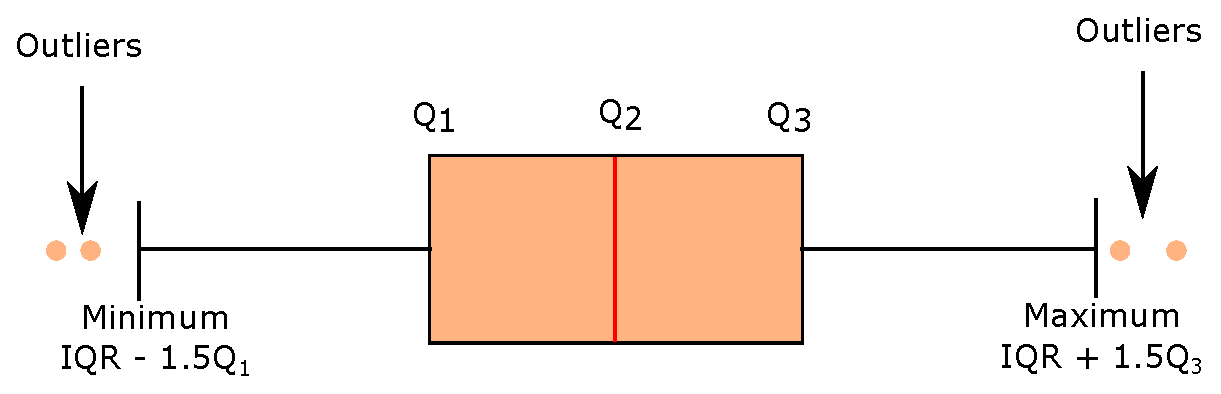
\includegraphics[width=0.5\linewidth]{./images/box_whisker_plot.eps}
		\caption{Box and Whisker Plot}
		\label{box_whisker_plot_example}
	\end{figure}
\end{tcolorbox}

\section{Histogram}
\begin{itemize}
	\item The purpose of a histogram (Chambers) is to graphically summarize the distribution of a univariate data set.
	\item The variable is divided into several bins or intervals, the number of observation per bin or interval is represented by the height of the bar
	\item A simple method to roughly calculate the number of bins or interval, is to take the square root of the total number of values in your distribution.
	\item The histogram graphically shows the following
	\begin{itemize}
		\item Center of the data
		\item Spread of the data
		\item Skewness of the data
		\item Presence of Outliers
		\item Presence of multiple Modes in the data 
	\end{itemize}
\end{itemize}

\begin{figure}[H]
	\centering
	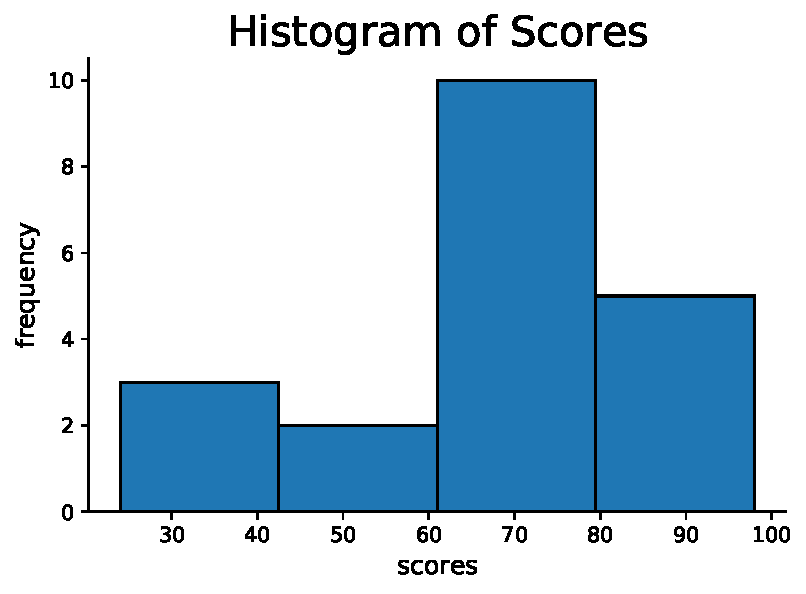
\includegraphics[width=0.5\linewidth]{./images/histogram_example.pdf}
	\caption{Example of histogram}
	\label{histogram_example}
\end{figure}

\vfill
\pagebreak
\section{Bar Graph}

A bar graph looks similar to histogram, however there is one key difference between them, bar graphs are used to visualize discrete data where as histograms are used for continuous data. A bar graph is shown in figure \ref{bargraph_example}


\begin{figure}[H]
	\centering
	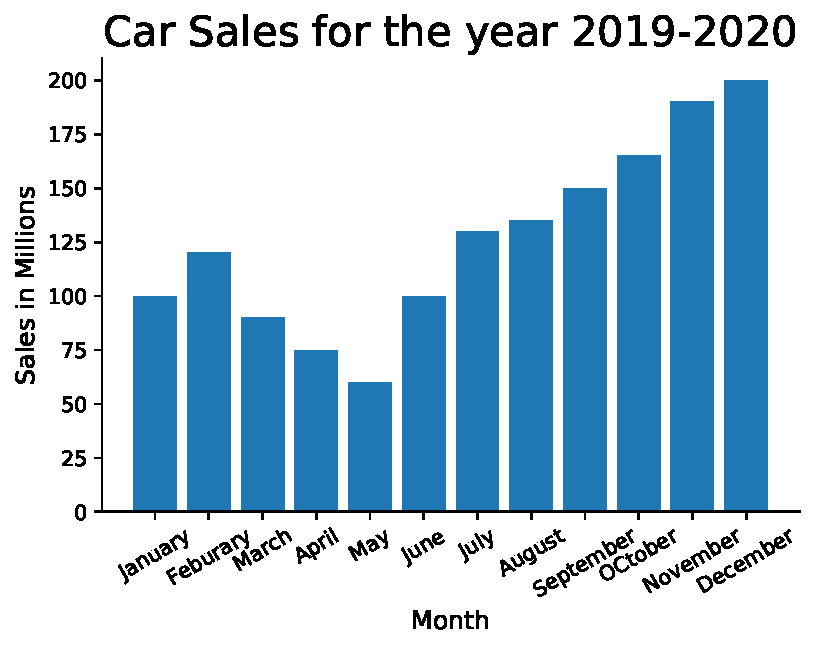
\includegraphics[width=0.5\linewidth]{./images/bargraph_example.pdf}
	\caption{Example of bar plot}
	\label{bargraph_example}
\end{figure}

\vfill
\pagebreak

\section{Line Graphs}

\begin{itemize}
	\item A line graph is typically used to visualize the change in variable over a period of time.
	\item It could also be used to represent the relationship between two variables
	\item When a Line Graph is used to visualize the change in variable over time it is known as \textbf{\textit{Run Sequence Plot}}
	\item With run sequence plots, shifts in location and scale are typically quite evident
	\item In Run Sequence Plot, outliers can be easily identified
\end{itemize}


\begin{figure}[H]
	\centering
	
	\begin{subfigure}[b]{0.5\textwidth}
		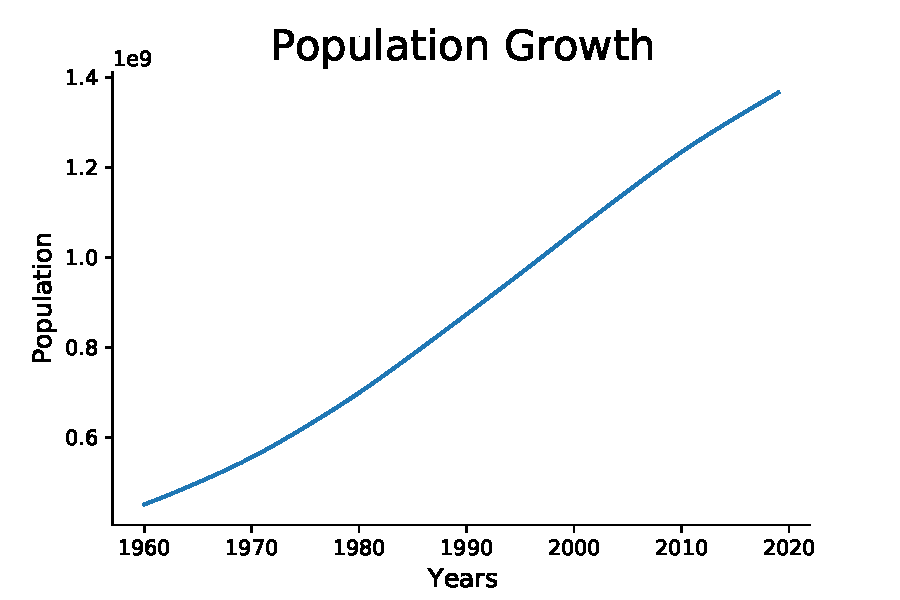
\includegraphics[width=\textwidth]{./images/linegraph_example.pdf}
		\subcaption{Univariate Line Graph}
		\label{linegraph_univariate_example}
	\end{subfigure}
	
	\begin{subfigure}[b]{0.3\textwidth}
		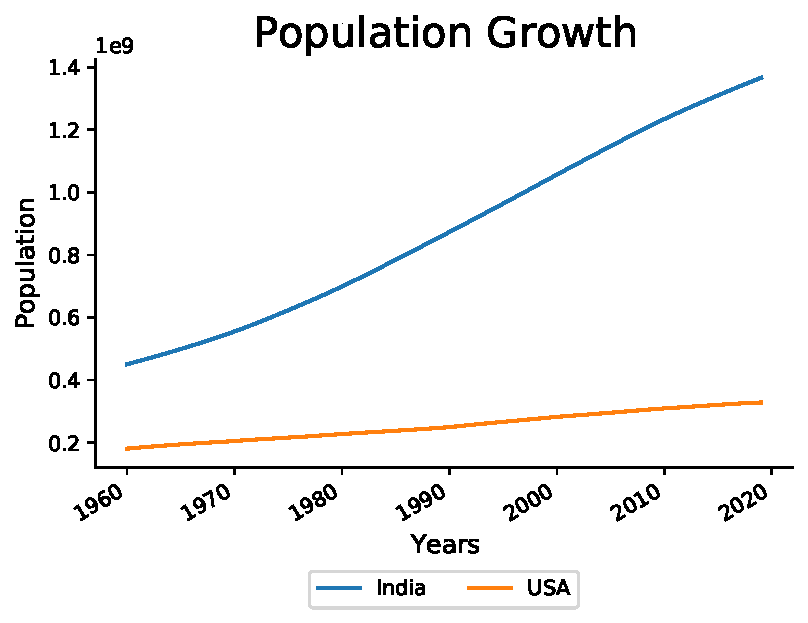
\includegraphics[width=\textwidth]{./images/linegraph_multivariate_example.pdf}
		\subcaption{Multivariate Line Graph}
		\label{line_graph_multivariate}
	\end{subfigure}
	\begin{subfigure}[b]{0.3\textwidth}
		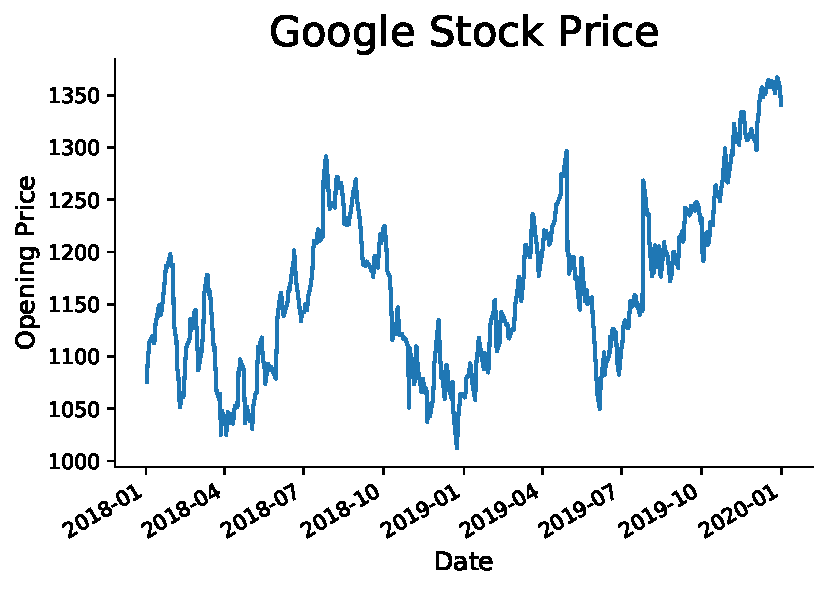
\includegraphics[width=\textwidth]{./images/run_sequence_example.pdf}
		\subcaption{Run Sequence Plot}
		\label{runsequence_example}
	\end{subfigure}
	\caption{Various Examples of Line Graphs}
	\label{line_graph_examples}
\end{figure}

\vfill

\pagebreak

\section{Pie Chart}
\begin{itemize}
	\item Unlike other charts and graphs, a pie is circular in nature
	\item It is often used to visualize proportions
	\item Various parameters like angle subtended by the arc at the center, length of the arc and area of the slice are proportional to the quantity it represents 
\end{itemize}

\begin{figure}[H]
	\centering
	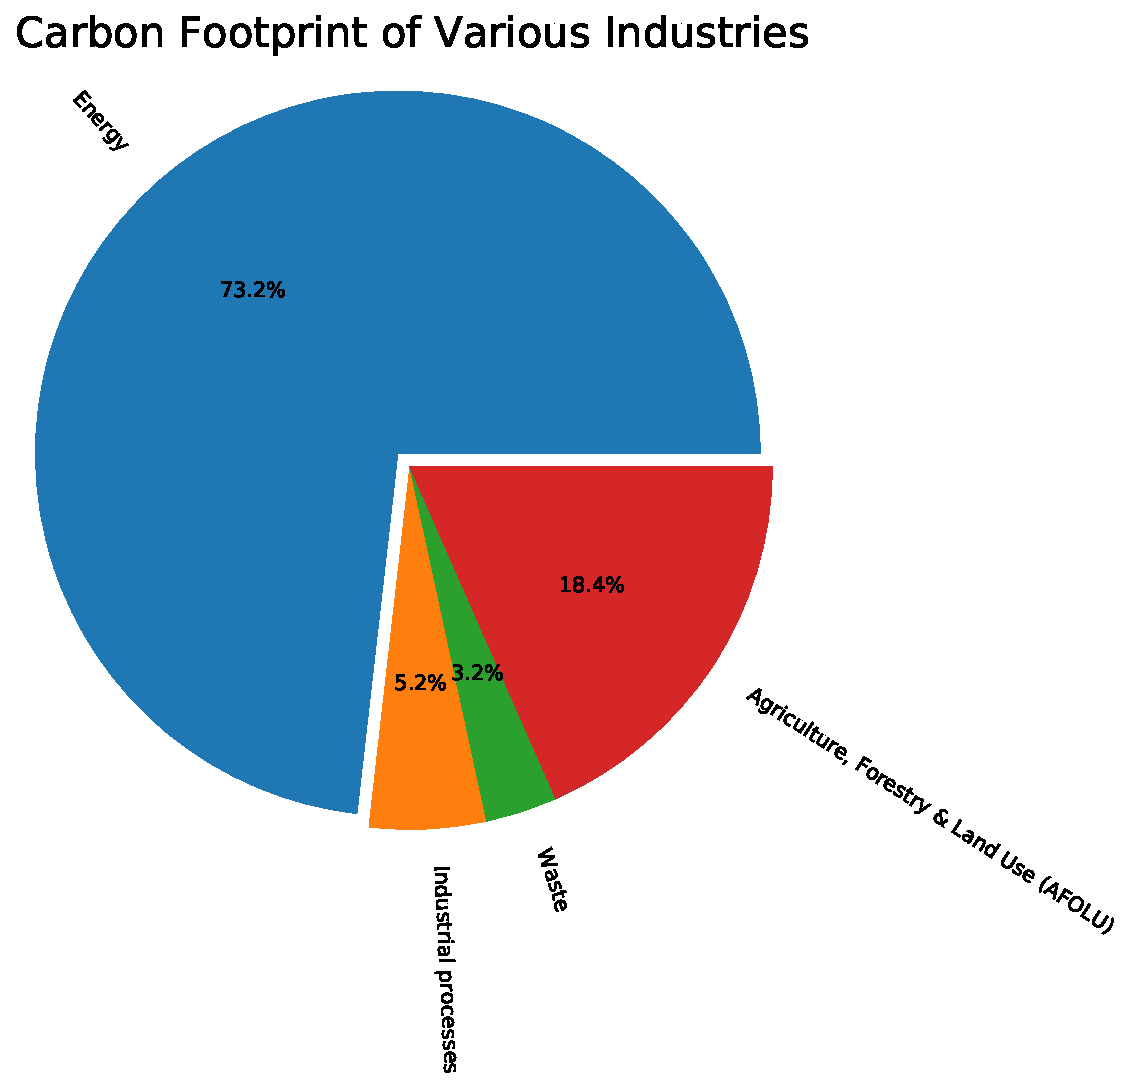
\includegraphics[width=0.5\linewidth]{./images/piechart_example.pdf}
	\caption{Example of Pie Chart}
	\label{piechart_example}
\end{figure}

\vfill

\pagebreak

\section{Scatter Plot}

Before proceeding further, we must familiarize ourselves with \textbf{covariance} and \textbf{correlation}

\subsection{What is Covariance ?}

\begin{tcolorbox}[colback=red!5!white, colframe=red!75!black, title = \textbf{Covariance}]
	Covariance is a measure of relation between the two variables which indicates the direction of linear relationship between variables. Covariance can be calculated as:
	$$ \boxed{cov(x,y) = \frac{\sum(x-\bar{x})(y-\bar{y})}{n}}$$
	\nomenclature[A]{$cov(x,y)$}{covarince of x and y}
\end{tcolorbox}
\noindent
\\
Covariance can indicate the following about the data:
\begin{itemize}
	\item A positive covariance indicates that increasing $x$ will result in a higher value of $y$ and decreasing $x$ will result in a lower value of $y$
	\item A negative correlation indicates that increasing $x$ will result in a lower value of $y$ and decreasing $x$ will result in a higher value of $y$
	\item If the covariance is zero it indicates that either decreasing or increasing the value of $x$ does not have any effect on $y$
\end{itemize}
\noindent
Covariance is not often used in statistics since it is hard to interpret due to the following reasons:
\begin{itemize}
	\item It does not gives much information about the slope of relationship
	\item It does not gives much information about relative position of data points
\end{itemize}

\subsection{What is Correlation ?}

\begin{tcolorbox}[colback=red!5!white, colframe=red!75!black, title = \textbf{Covariance}]
	Correlation is a measure of strength and direction between two variables. Correlation can be calculated as:
	$$ \boxed{corr(x,y) = \frac{cov(x,y)}{\sigma_{x}\sigma_{y}}} $$
	\nomenclature[A]{$corr(x,y)$}{Correlation between x and y}
\end{tcolorbox}
\noindent
\\
For a better understanding of correlation, let us imagine a following scenario. Let us imagine a straight line given by equation $y=mx+c$, where $x$ and $y$ represents the $x$ and $y$ coordinate respectively, $m$ is the slope and $c$ represents y-intercept. For this scenario the following holds true:
\begin{itemize}
	\item For every point on the line there is a strong correlation between the points on $x$ and $y$
	\item The nature of correlation depends on the slope of the line
\end{itemize} 
\noindent
For the above scenario the correlation between the points on x and y-axis will be either -1 or 1 based on the nature of the slope. A correlation of -1 or 1 means for any given value of x the corresponding y value will be linearly related. Now let us imagine that few points are slightly displaced from their location such that they do not follow strict linear relationship, for this dataset the value of correlation will not be 1 or -1 the value will decrease based on the amount of displacement from from the original location. 

\subsection{What are Scatter Plots?}

\begin{itemize}
	\item Scatter plots are used to observe relationships between variables
	\item A scatter plot (aka scatter chart, scatter graph) uses dots to represent values for two different numeric variables
	\item The position of each dot on the horizontal and vertical axis indicates values for an individual data point
\end{itemize}

\begin{figure}[H]
	\centering
	
	\begin{subfigure}[b]{0.25\textwidth}
		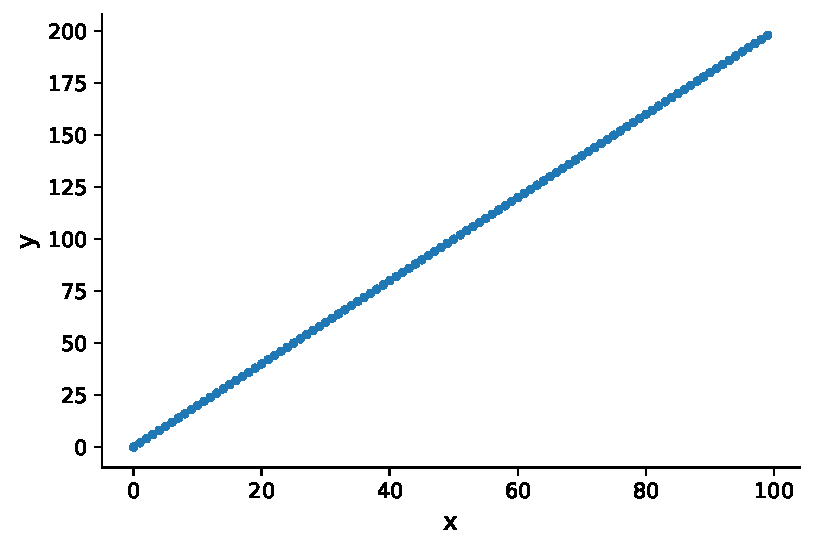
\includegraphics[width=\textwidth]{./images/scatterplot_strong_positive_example.pdf}
		\subcaption{Strong Positive Correlation}
		\label{scatterplot_example_strong_positive}
	\end{subfigure}
	\begin{subfigure}[b]{0.25\textwidth}
		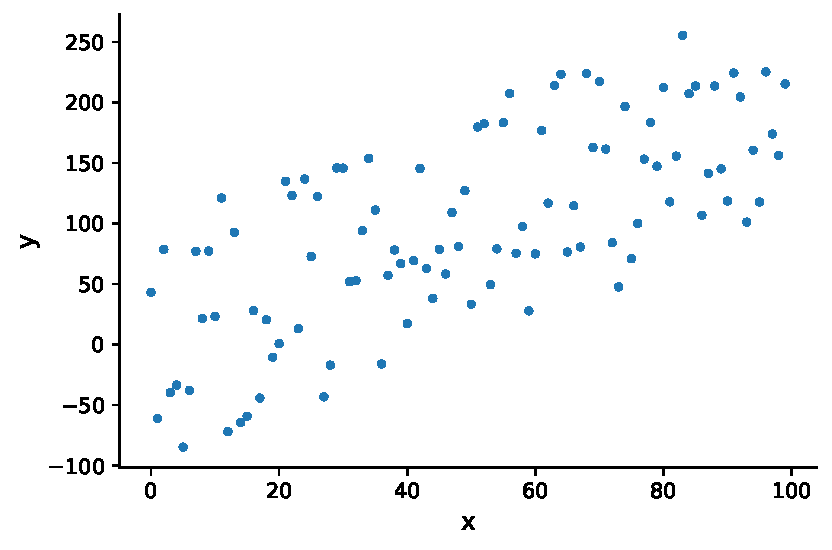
\includegraphics[width=\textwidth]{./images/scatterplot_weak_positive_example.pdf}
		\subcaption{Weak Positive Correlation}
		\label{scatterplot_example_weak_positive}
	\end{subfigure}
	
	\begin{subfigure}[b]{0.25\textwidth}
		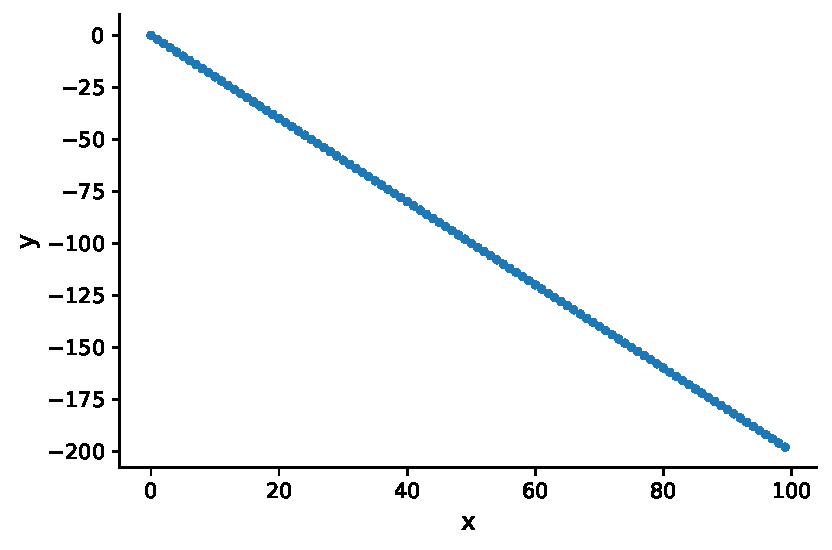
\includegraphics[width=\textwidth]{./images/scatterplot_strong_negitive_example.pdf}
		\subcaption{Strong Negative Correlation}
		\label{scatterplot_example_strong_negative}
	\end{subfigure}
	\begin{subfigure}[b]{0.25\textwidth}
		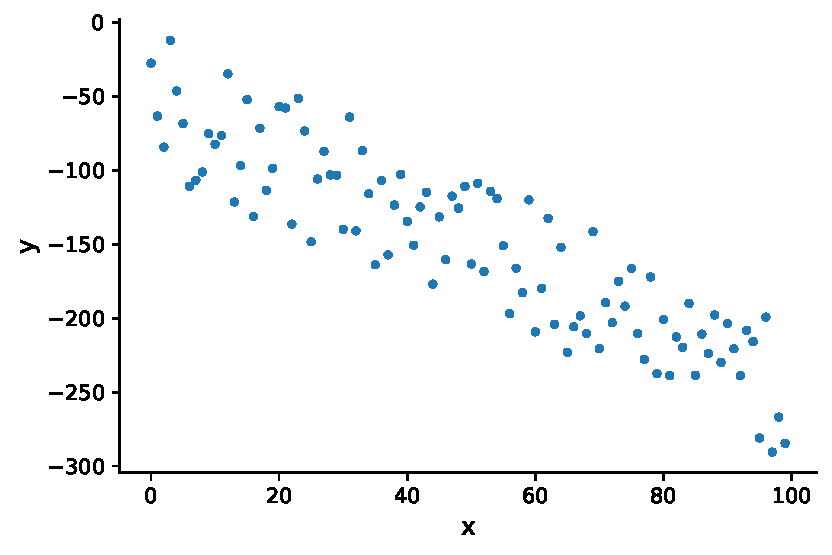
\includegraphics[width=\textwidth]{./images/scatterplot_weak_negitive_example.pdf}
		\subcaption{Weak Negitive Correlation}
		\label{scatterplot_example_weak_negative}
	\end{subfigure}
	\caption{Examples of Scatter Plots}
	\label{scatterplot_example}
\end{figure}

\vfill
\pagebreak

\section{Heat Map}

\begin{tcolorbox}[colback=red!5!white, colframe=red!75!black, title = \textbf{Heat Map}]
	A Heat Map is a method of visualizing the values in 2D matrix. The magnitude of the value is represented by a color taken from a colormap.
\end{tcolorbox}
\noindent
\\
Heat maps are most widely used for visualizing correlation between variables, hence it usually has the same number of rows and columns. \textbf{\textit{It must be noted that when a heat map is used for visualizing  correlation, the diagonals always have a value of 1 because they represent the relation of a column with itself.}}

\begin{figure}[H]
	
	\centering
	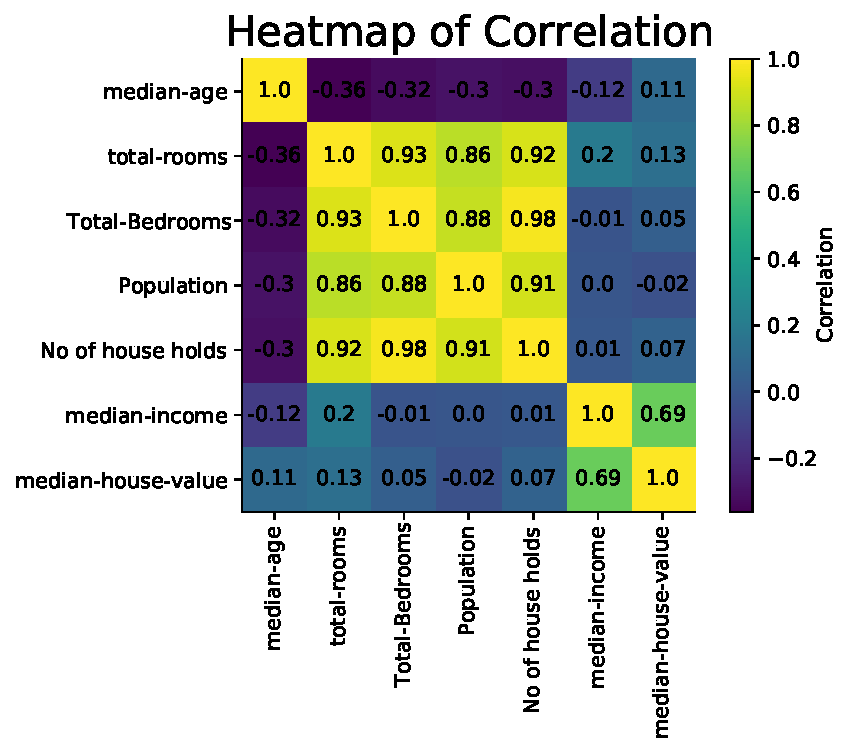
\includegraphics[width=0.5\linewidth]{./images/heatmap_example.pdf}
	\caption{Example of Heat Map}
	\label{heatmap_example}

\end{figure}
\noindent
We will now proceed with a slightly more advance concept of \textbf{\textit{Pareto Chart}}

\section{Pareto Chart}

Pareto Charts are based on \textbf{\textit{Pareto Principal}}, hence it imperative that we first familiarize ourself with Pareto Principal
\\
\begin{tcolorbox}[colback=red!5!white, colframe=red!75!black, title = \textbf{Pareto Principal}]
	The Pareto principle (also known as the 80/20 rule, the law of the vital few, or the principle of factor sparsity) states that, for many events, roughly 80\% of the effects come from 20\% of the causes
\end{tcolorbox}
\noindent
\\
A \textbf{\textit{Pareto Chart}} is a combination of  Line Graph and Bar Plot as we will see in the example below.

\begin{tcolorbox}[colback=blue!5!white, colframe=blue!75!black, title = \textbf{Pareto Chart}]
	
	Let us suppose we have the data given in table \ref{pareto_example_table}. This data can be converted to a Pareto Chart using the following steps:
	\begin{enumerate}
		\item \textbf{Arrange the data in descending order} 
		\item \textbf{Plot the bar graph} 
		\item \textbf{Calculate cumulative percentage :} To calculate cumulative percentage, we first need to calculate cumulative frequency, then cumulative frequency for each category is divided by total and multiplied by 100. For ex: To calculate the cummulative frequency of Electrical Defects we will divide 687 by 754 and multiply by 100, i.e. $ \mbox{cumulative frequency of Electrical Defects} = \frac{687}{754} \times 100 = 91.11 $
		\item \textbf{Plot line graph :} Line graph is plotted to represent cumulative percentage of each category	
	\end{enumerate}

	\begin{table}[H]
		\begin{centering}
			\begin{tabular}{c|c|c|c}
				\textbf{Types of   Defects} &\textbf{Frequency} &\textbf{Cummulative Frequency} &\textbf{Cummulative Percentage} \\
				\hline
				Panel Gaps                  & 200                & 200                              & 26.53 \\
				Paint Defects               & 123                & 323                              & 42.84 \\
				Electrical Defects          & 364                & 687                              & 91.11 \\
				Major Mechanical Defects    & 10                 & 697                              & 92.44 \\
				Minor Fixture Issues        & 57                 & 754                              & 100.00 \\        
			\end{tabular}
			\caption{Types of Defects reported by a car manufacturer}
			\label{pareto_example_table}
		\end{centering}
	\end{table}

	\begin{figure}[H]
		\centering
		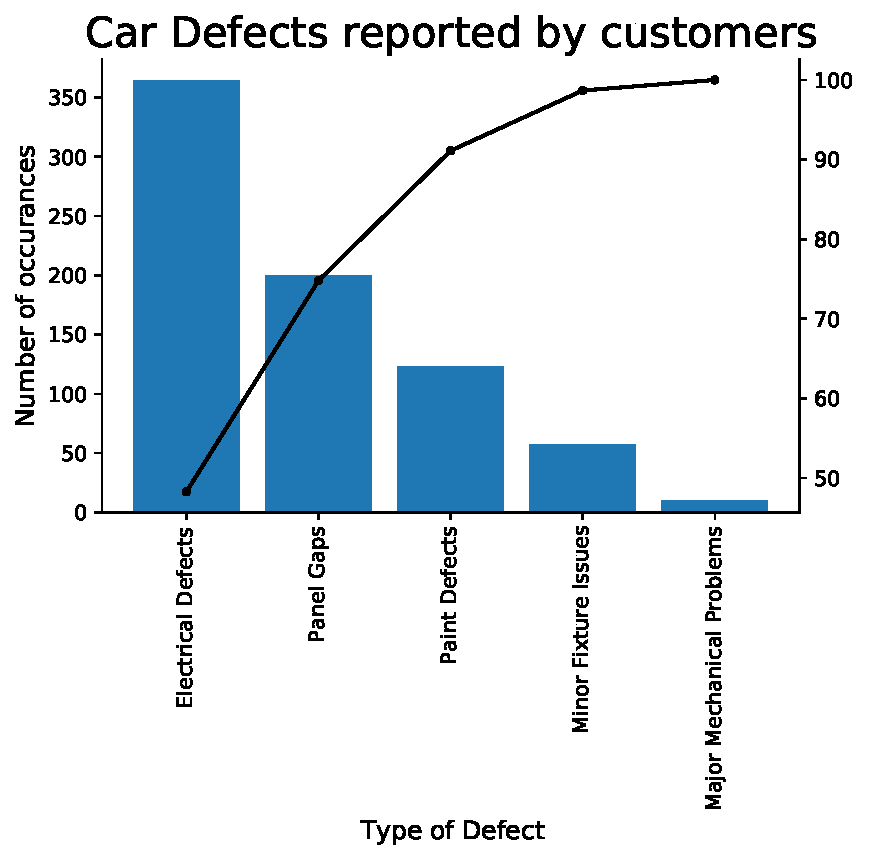
\includegraphics[width=0.5\linewidth]{./images/paretochart_example.pdf}
		\caption{Example of Pareto Chart}
		\label{paretochart_example}
	\end{figure}

\end{tcolorbox}

%%%%%%%%%%%%%%%%%%%%%%%%%%%%%%%%%%%%%%%%%%%%%%%%%%%%%%%%%%%%%%%%%%%%%%%%%%%%%%%%%%%%%%%%%%%%%%%%%%%%%%%%%%%%%%%%%%%%%%%%%%%%%%%%%%%%%%%%%%%%%%%%%%%%%%%%%%%%%%%%%%%%%%%%%%%%%%%%%%%%%%%%%%%%%%%%%%%

\chapter{Probability}

\section{What is Probability ?}

\begin{tcolorbox}[colback=red!5!white, colframe=red!75!black, title = \textbf{Probability}]
	Probability means chance. It can be mathematically expressed as
	$$ P = \frac{\mbox{favourable outcome}}{\mbox{total number of outcomes}} $$
	\nomenclature[A]{$P$}{Probability}
	We can also say that Probability is the ratio of favorable outcome to possible outcomes
\end{tcolorbox}
\noindent
\\
Let us take an example to understand this concept

\begin{tcolorbox}[colback=blue!5!white, colframe=blue!75!black, title = \textbf{Probability}]
	What is the probability of drawing a club from a deck of cards.
	$$\mbox{Favourable outcome} = \mbox{number of club cards in a deck} = 13$$
	$$\mbox{Total Number of outcome} = \mbox{Total number of cards in a deck} = 52$$
	$$ P = \frac{13}{52} = \frac{1}{4} = 0.25$$
	
	There is 25\% probability that the card drawn will a club card
\end{tcolorbox}

\section{Basic Terminology of Probability}

To fully understand probability the reader first need to familiarize itself with the basic terminology used in in Probability. Before proceeding further we need to familiarize ourselves with the following terms:
\begin{itemize}
	\item Probability Experiment
	\item Events
	\item Outcomes
	\item Sample Space
\end{itemize}

\subsection{Probability Experiment}

\begin{tcolorbox}[colback=red!5!white, colframe=red!75!black, title = \textbf{Probability Experiment}]
	A repeatable experiment with defined set of outcomes is called a Probability Experiment	
\end{tcolorbox}

\subsection{Outcomes}
\begin{tcolorbox}[colback=red!5!white, colframe=red!75!black, title = \textbf{Outcomes}]
	The result of a probability experiment is known as outcome
\end{tcolorbox}


\subsection{Sample Space}
\begin{tcolorbox}[colback=red!5!white, colframe=red!75!black, title = \textbf{Sample Space}]
	Collection of all possible outcomes of a probability experiment is known as Sample Space
\end{tcolorbox}

\subsection{Events}
\begin{tcolorbox}[colback=red!5!white, colframe=red!75!black, title = \textbf{Events}]
	A collection of a few outcomes from sample space is known as an event. It is a subset of sample space.
\end{tcolorbox}
\noindent
\\
\begin{tcolorbox}[colback=blue!5!white, colframe=blue!75!black, title = \textbf{Probability Experiment, Outcomes, Sample Space, Events}]
	Let us consider that a fair coin is tossed 2 times, then we can say that
	\\
	\\
	Tossing of coin itself is the \textbf{probability experiment}.
	\\
	\\
	Occurrence of Heads or Tails are the two \textbf{outcomes}
	\\
	\\
	The \textbf{Sample Space} can be expressed as \{HH\}, \{TT\}, \{HT\}, \{TH\}. 
	\\
	\\
	We can have the following events:
	
	\begin{table}[H]
		\centering
		\begin{tabular}{c|c}
			\textbf{Event}   & \textbf{Outcomes}       \\
			\hline
			1 Head  & \{HT\}, \{TH\} \\
			1 Tail  & \{HT\}, \{TH\} \\
			2 heds  & \{HH\}         \\
			2 Tails & \{TT\}     
		\end{tabular}
		\caption{Possible Events and Outcomes form tossing of a coin}
		\label{table_tossing _of_coin}
	\end{table}
\end{tcolorbox}
\section{Union and Intersection of Events}

\begin{tcolorbox}[colback=red!5!white, colframe=red!75!black, title = \textbf{Union of Events}]
	In case of two distinct events A and B, the union of the event will contain all the outcomes that are present in either A or B. The union of two events is represented as $A \bigcup B$.
\end{tcolorbox}

\vfill

\begin{tcolorbox}[colback=red!5!white, colframe=red!75!black, title = \textbf{Intersection of Events}]
	In case of two distinct events A and B, the intersection of the events will contain all the elements present in both A and B. The union of two events is represented as $ A \bigcap B $ 
\end{tcolorbox}
\noindent
\\
\begin{tcolorbox}[colback=blue!5!white, colframe=blue!75!black, title = \textbf{Union and Intersection of Events}]
	Let us consider two events A and B having the following outcomes from rolling of a dice:
	\\
	Event A = $\{2,4,6\}$
	\\
	Event B = $\{3,6\}$
	\\
	Event(A $\bigcup$ B) = $\{2,3,4,6\}$
	\\
	Event(A $\bigcap$ B) = $\{6\}$	
\end{tcolorbox}

\section{Types of Events}

\subsection{Mutually Exclusive Events}

\begin{tcolorbox}[colback=red!5!white, colframe=red!75!black, title = \textbf{Mutually Exclusive Events}]
	Two events are said to be mutually exclusive if the occurrence of one event implies that other event event will not occur.
\end{tcolorbox}
\noindent
\\

\begin{tcolorbox}[colback=blue!5!white, colframe=blue!75!black, title = \textbf{Mutually Exclusive Events}]
	Occurrence of head or tail are mutually exclusive events because occurance of one confirms that the other will not occur.
\end{tcolorbox}
\noindent
\\
\noindent
\textbf{It must be noted that for mutually exclusive events A and B, $ \boldsymbol{P(A \bigcap B) = 0} $}

\subsection{Non Mutually Exclusive Events}

\begin{tcolorbox}[colback=red!5!white, colframe=red!75!black, title = \textbf{Non Mutually Exclusive Events}]
	Two events are said to be non-mutually exclusive if they can occur  together 
\end{tcolorbox}
\noindent
\\
\begin{tcolorbox}[colback=blue!5!white, colframe=blue!75!black, title = \textbf{Non-Mutually exclusive Event}]
	A single card drawn from a deck of cards could be both an ace and a club card at the same time. Thus we can say that drawing a club card and drawing an ace are non-mutually exclusive events
\end{tcolorbox}
\noindent
\\
\subsection{Independent Events}

\begin{tcolorbox}[colback=red!5!white, colframe=red!75!black, title = \textbf{Independent Events}]
	Two Events are said to be independent  if the occurrence of one event does not affects the probability of occurrence of the other  
\end{tcolorbox}
\noindent
\\
\begin{tcolorbox}[colback=blue!5!white, colframe=blue!75!black, title = \textbf{Independent Events}]
	Two consecutive rolls of a fair dice.
\end{tcolorbox}
\noindent
\\
\subsection{Dependent Events}

\begin{tcolorbox}[colback=red!5!white, colframe=red!75!black, title = \textbf{Dependent Events}]
	Two events are said to be dependent if occurrence of one event does affects the probability of occurrence of another event
\end{tcolorbox}
\noindent
\\
\begin{tcolorbox}[colback=blue!5!white, colframe=blue!75!black, title = \textbf{Dependent Events}]
	Let us imagine a box of fruits containing 5 apples, 5 bananas and 5 oranges. Let us say we randomly pick a fruit from the box. Then we pick another fruit without replacing the fruit we picked earlier, this will affect the next outcome.
	\\
	\\
	Let us look at this from a mathematical point of view.
	\\
	\\
	Probability of picking an orange in the first go is $ \frac{5}{15} $
	\\
	Let us now randomly draw a fruit from the box, let this fruit be a banana, thus probability of drawing an orange in the second go is $ \frac{5}{14} $ because we have not replaced the fruit we have drawn in the first draw.
\end{tcolorbox}
\noindent
\\
\section{Rules of Probability}

\begin{enumerate}
	\item $ P(A^{C}) = 1 - P(A) $
	\item $ A \subset B \Longrightarrow P(A) \le P(B)$
	\item $ P(A \bigcup B) = P(\mbox{A or B}) = P(A) + P(B) - P(A \bigcap B) $
	\item $ P(A \bigcup B \bigcup C) = P(A) + P(B) + P(C) - P(A \bigcap B) - P(A \bigcap C) - P(B \bigcap C) + 2P(A \bigcap B \bigcap C) $
	\item If A and B are independent events than $P(\mbox{A and B}) = P(A \bigcap B) = P(A) \times P(B)$
\end{enumerate}

\begin{tcolorbox}[colback=blue!5!white, colframe=blue!75!black, title = \textbf{Union and Intersection of Two Sets}]
	In a class of engineering freshmen, there is a 80 percent chance that a student will opt for advance physics during the next semester, there is 60 percent chance that a student will opt for advance maths and there is 50 percent chance that a student will opt for both. Given a student is selected at random what is the probability that he/she will opt for either advance physics or advance maths ?
	\\
	\\
	Let A be the probability that student selects advance physics and let B be the probability that student selects advance maths i.e.
	$$ P(A) = \mbox{P(Advance Physics)} = \frac{80}{100} $$
	$$ P(B) = \mbox{P(Advance Maths)} = \frac{60}{100} $$
	$$ P(A \bigcap B) = \mbox{P(Advance Maths \& Advance Physics)} = \frac{50}{100} $$
	$$ P(A \bigcup B) =P(A) + P(B) - P(A \bigcap B) $$
	$$ P(A \bigcup B) = \frac{80}{100} + \frac{60}{100} - \frac{50}{100}  $$
	$$ P(A \bigcup B) = \frac{90}{100}  $$
	\\
	There is 90 percent chance that a student selected at random will select either Advance Physics or Advance Maths. 
	
	\begin{figure}[H]
		\centering
		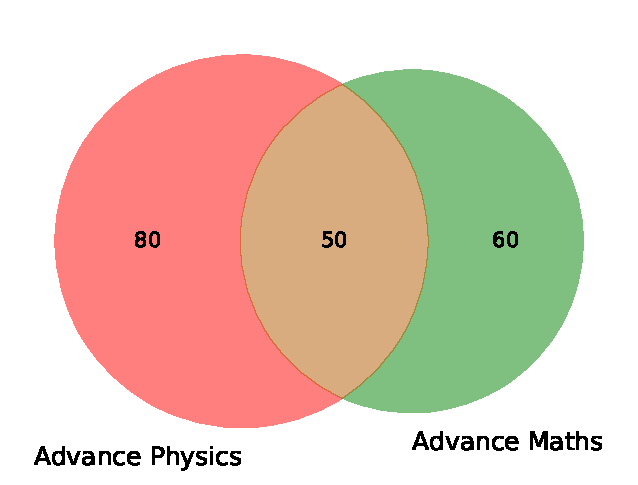
\includegraphics[width=0.5\linewidth]{./images/figure_venn2.pdf}
		\caption{Venn Diagram of Probabilities for Two Events}
		\label{venn2}
	\end{figure}
\end{tcolorbox}

\vfill
\pagebreak

\begin{tcolorbox}[colback=blue!5!white, colframe=blue!75!black, title = \textbf{Union and Intersection of Three Sets}]
	In a survey conducted on high school class it was observed that if a student is selected at random, then there is 30 percent probability that he/she is studying  physics as major, 45 percent probablity that he/she is studying chemistry as major and 60 percent probability that he/she is studying maths as major. There is 15 percent probability that a student is majoring in both physics and chemistry, 30 percent probability that a student is majoring in both physics and maths, and 20 percent probability that a student is majoring in chemistry and maths. If the there is 80 percent probability that a student selected at random is majoring in either in physics, chemistry or maths is 80 percent. Calculate the probability that a student selected at random will be majoring in all three subjects.
	\\
	\\
	Let
	$$ P(A) = P(\mbox{Physics}) = \frac{30}{100} $$
	$$ P(B) = P(\mbox{Chemistry}) = \frac{45}{100} $$
	$$ P(C) = P(\mbox{Maths}) = \frac{60}{100} $$
	$$ P(A \bigcap B) = \frac{15}{100} $$
	$$ P(A \bigcap C) = \frac{30}{100} $$
	$$ P(B \bigcap C) = \frac{20}{100} $$
	$$ P(A \bigcup B \bigcup C) = \frac{80}{100} $$
	We know that
	$$ P(A \bigcup B \bigcup C) =  P(A) + P(B) + P(C) - P(A \bigcap B) - P(A \bigcap C) - P(B \bigcap C) + 2P(A \bigcap B \bigcap  C) $$
	$$ \frac{80}{100} = \frac{30}{100} + \frac{45}{100} + \frac{60}{100} - \frac{15}{100} - \frac{30}{100} - \frac{20}{100} + 2P(A \bigcap B \bigcap C) $$
	$$ \frac{80}{100} = \frac{135}{100} - \frac{65}{100} + 2P(A \bigcap B \bigcap C) $$
	$$ \frac{80}{100} = \frac{70}{100} + 2P(A \bigcap B \bigcap C) $$
	$$P(A \bigcap B \bigcap C) = \frac{5}{100}$$
	
	Thus there is 5 percent probability that a student selected at random will be majoring in physics, chemistry and maths.
\end{tcolorbox}

\vfill
\pagebreak

\section{Types of Probability}

\subsection{Marginal Probability}

\begin{tcolorbox}[colback=red!5!white, colframe=red!75!black, title = \textbf{Marginal Probability}]
	The probability of occurrence of a single event is called marginal probability
\end{tcolorbox}
\noindent
\\
\begin{tcolorbox}[colback=blue!5!white, colframe=blue!75!black, title = \textbf{Marginal Probability}]
	The probability of occurrence of a an even number when a fair dice is rolled a single time.
\end{tcolorbox}
\noindent
\\
\subsection{Joint Probability}

\begin{tcolorbox}[colback=red!5!white, colframe=red!75!black, title = \textbf{Joint Probability}]
	The Probability of occurrence of two events at the same time is known as joint probability
\end{tcolorbox}
\noindent
\\
Joint Probability has the following properties:
\begin{itemize}
	\item Joint Probability of two independent events A and B can be calculated as
	$$ P(A \bigcap B) = P(A) \times P(B)$$
	\item Joint Probability of dependent events can't be calculated
\end{itemize}

\begin{tcolorbox}[colback=blue!5!white, colframe=blue!75!black, title = \textbf{Joint Probability}]
	A box contains 5 red and 3 blue marbles, calculate the probability that the first marble drawn is red and the second marble is blue if the marbles are drawn successively without replacing.
	\\
	\\
	 $$ P(A) = P(\mbox{Drawing a red marble}) = \frac{5}{8}$$
	 $$ P(B) = P(\mbox{Drawing a blue marble}) = \frac{3}{7} $$
	 $$ P(A \bigcap b) = P(A) \times P(B) = \frac{5}{8} \times \frac{3}{7} = \frac{15}{56} $$
\end{tcolorbox}
\noindent
\\
\subsection{Conditional Probability}

\begin{tcolorbox}[colback=red!5!white, colframe=red!75!black, title = \textbf{Conditional Probability}]
	Conditional Probability is the probability of a dependent event A occurring given that another event B has already occurred
\end{tcolorbox}
\noindent
\\
Conditional probability of Event A occuring given that event B has already occurred is expressed as
\begin{center}
	\boxed{$$ P(A|B) = \frac{P(\mbox{A and B})}{P(B)} = \frac{P(A \bigcap B)}{P(B)} $$ }
\end{center}

\begin{tcolorbox}[colback=blue!5!white, colframe=blue!75!black, title = \textbf{Conditional Probability}]
	Calculate the conditional probability of successively drawing two kings from a deck of cards without replacing.
	\\
	Let
	$$ P(A) = P(\mbox{Drawing the first king}) = \frac{4}{52} $$
	$$ P(B) = P(\mbox{Drawing the second king}) = \frac{3}{51} $$
	$$ P(\mbox{A and B}) = P(A) \times P(B) = \frac{4}{52} \times \frac{3}{51} $$
	$$ P(A|B) = \frac{P(A \bigcap B)}{P(B)} = \frac{\frac{4}{52} \times \frac{3}{51}}{\frac{4}{52}} = \frac{3}{51} $$
\end{tcolorbox}
\noindent
\\
\section{Odds and Log of Odds}

\subsection{Odds}
\begin{tcolorbox}[colback=red!5!white, colframe=red!75!black, title = \textbf{Odds}]
	Odds of an Event A are the ratio of outcomes . Odds in favour of Event A is the ratio of favorable outcomes to the ratio of unfavorable outcomes. Odds against Event A is the ratio of unfavorable outcomes to the ratio of favorable outcomes. Odds can be mathematically expressed as
	$$ \mbox{Odds in favour of A} = \frac{\mbox{Number of favourable outcomes}}{\mbox{Number of unfavourable outcomes}} $$ 
	$$ \mbox{Odds against A} = \frac{\mbox{Number of unfavourable outcomes}}{\mbox{Number of favourable outcomes}} $$ 
\end{tcolorbox}
\noindent
\\
\begin{tcolorbox}[colback=blue!5!white, colframe=blue!75!black, title = \textbf{Odds}]
	What are the odds of drawing an ace from a deck of cards ?
	$$ \mbox{Favourable outcomes} = 4 $$
	$$ \mbox{Unfavourable Outcomes} = 52 - 4 = 48 $$
	$$ \mbox{Odds in favour} = \frac{4}{48} $$
	$$ \mbox{Odds against} = \frac{48}{4} $$
\end{tcolorbox}
\noindent
\\
\subsection{Log of Odds}

\begin{tcolorbox}[colback=red!5!white, colframe=red!75!black, title = \textbf{Log of Odds}]
	Log of Odds is the logarithmic of odds
\end{tcolorbox}
\noindent
\\
\section{Baye's Theorem}

A formal definition of Baye's theorem at this point will be complicated to interpret as it requires the understanding of certain concepts and principals which have not been covered, hence we will take a slightly different approach to understand the driving ideas behind Baye's Theorem.
\\
\\
In the previous section we discovered what is conditional probability. The notion $P(A|B)$ denotes the probability of event A occurring given that event B has already occurred.
\\
\\
Let us assume that there exist two events named A and B. Let us assume the following probabilities are known:
\begin{itemize}
	\item $ P(A \bigcap B) $
	\item $ P(B) $
\end{itemize}
\noindent
Using the above data we can clearly determine the probability of Event A given that Event B has already occurred. But what if we have to determine the probability of Event B given that Event A has already occurred.
\\
\\
This is where Baye's Theorem comes into picture. \textbf{Baye's Theorem is used to analyze how well a proof fits a theory.} Let us familiarize ourselves with this concept with the help of an example.
\\
\\
Let us assume a group of individuals who are inhabitants of different states of USA. It is theorized that 30 percent of individuals from the state of Texas are farmers, 20 percent of all the individuals are farmers and 40 percent individuals are from Texas.
\\
\\
We can mathematically express it as
$$ P(A) = P(\mbox{Farmer}) = \frac{20}{100} = 0.2 $$
$$ P(B) = P(\mbox{Texas}) = \frac{40}{100} = 0.4$$
$$ P(A | B) = P(Farmer|Texas) = \frac{30}{100} = 0.3 $$
\\
Now let us assume that we need to calculate the probability of a person being from Texas given that he is a farmer i.e. $P(B|A)$.
\\
\\
Thus using Baye's Theorem we can use the following relation
\begin{center}
	\boxed{$$ P(B|A) = \frac{P(A|B)P(B)}{P(A)} $$}
\end{center}
\noindent
Thus based on the above theorem we can say that
$$ P(Texas|Farmer) = \frac{P(Farmer|Texas)P(Texas)}{P(Farmer)} $$
$$ P(B|A) = \frac{0.3 \times 0.4}{0.2} = 0.6 $$
\\
As can be seen that there is 60 percent probability that if a farmer is selected he/she is a resident of Texas.
%%%%%%%%%%%%%%%%%%%%%%%%%%%%%%%%%%%%%%%%%%%%%%%%%%%%%%%%%%%%%%%%%%%%%%%%%%%%%%%%%%%%%%%%%%%%%%%%%%%%%%%%%%%%%%%%%%%%%%%%%%%%%%%%%%%%%%%%%%%%%%%%%%%%%%%%%%%%%%%%%%%%%%%%%%%%%%%%%%%%%%%%%%%%%%%%%%%
\chapter{Probability Distribution}
\noindent
Before exploring the more advance concepts of probability, familirity with the term \textbf{\textit{Random Experiment}} and \textbf{\textit{Random Variable}} is required. Hence we will first explore these concepts
\\
\begin{tcolorbox}[colback=red!5!white, colframe=red!75!black, title = \textbf{Random Experiment}]
	A random experiment is a experiment whose outcome cannot be predicted with absolute certainty.
\end{tcolorbox}
\noindent
\break
\begin{tcolorbox}[colback=red!5!white, colframe=red!75!black, title = \textbf{Random Variable}]
	A random variable is real valued function which can take up any value from the sample space of Random Experiment. 
\end{tcolorbox}
\noindent
\\
\section{Types of Probability Distribution Functions}
\noindent
Before we proceed further we must familiarize ourselves with what is \textbf{\textit{probability distribution function}}
\\
\begin{tcolorbox}[colback=red!5!white, colframe=red!75!black, title = \textbf{Probability Distribution Function}]
	Probability distribution is a list of all outcomes of a random experiment along with their probabilities.
\end{tcolorbox}
\noindent
\\
In order to better understand this we need to understand different kinds of probability distribution functions. Probability distribution function can be classified into three categories:
\begin{itemize}
	\item Probability Mass Function
	\item Probability Density Function
	\item Cumulative Distribution Function
\end{itemize}


\subsection{Probability Mass Function}
\begin{tcolorbox}[colback=red!5!white, colframe=red!75!black, title = \textbf{Probability Mass Function}]
	A probability distribution function can be classified as probability mass function if the random variable can take only discreet values 
\end{tcolorbox}
\noindent
\\
To better understand this let us take an example

\begin{tcolorbox}[colback=blue!5!white, colframe=blue!75!black, title = \textbf{Probability Mass Function}]
	Let the random experiment be rolling of a dice . Then the random variable  $X$ can take values 1, 2, 3, 4, 5 and 6. 
	Then Probability Mass function will look like this
	\begin{table}[H]
		\centering
		\begin{tabular}{c|c}
			$\boldsymbol{X=x}$ & $\boldsymbol{P(X=x)}$      \\
			\hline
			1     & $\frac{1}{6}$ \\
			2     & $\frac{1}{6}$ \\
			3     & $\frac{1}{6}$ \\
			4     & $\frac{1}{6}$ \\
			5     & $\frac{1}{6}$ \\
			6     & $\frac{1}{6}$
		\end{tabular}
		\caption{Probability Mass Function for rolling of a dice}
		\label{probability_mass_function_example}
	\end{table}
\end{tcolorbox}

\subsection{Probability Density Function}

\begin{tcolorbox}[colback=red!5!white, colframe=red!75!black, title = \textbf{Probability Density Function}]
	A probability distribution function can be classified as probability density function if the random variable can take only continuous values.
\end{tcolorbox}
\noindent
\\
In simple words we can say that Probability Density Function can predict the probability of random variable X falling within a specific range within the sample space i.e. it can be mathematically expressed as
$$ P(a \le X \le b) = \int_{a}^{b} f(x) $$
\noindent
\textbf{It must be noted that probability function for probability density function is an integral, this is because of the nature of random variable} 
\\
\begin{tcolorbox}[colback=blue!5!white, colframe=blue!75!black, title = \textbf{Probability Density Function}]
	Let us consider a dataset consisting of height of individuals as shown in table \ref{table_probabilitydensityfunction_example}.
	
	\begin{table}[H]
		\centering
		\begin{tabular}{c|c}
			\textbf{Height in ft} & \textbf{Frequency} \\
			\hline
			2.5 - 3.5       & 23                 \\
			3.5 - 4.5       & 135                \\
			4.5 - 5.5       & 340                \\
			5.5 - 6.5       & 340                \\
			6.5 - 7.5       & 135                \\
			7.5 - 8.5       & 23                
		\end{tabular}
		\caption{Probability Density Function for Height of people}
		\label{table_probabilitydensityfunction_example}
	\end{table}
	
	The above table can be interpreted as follows, if we randomly select an individual from the dataset shown in table \ref{table_probabilitydensityfunction_example} then there is $\frac{640}{960}$ chance that the person will have a height between 4.5 and 6.5 ft.
\end{tcolorbox}

\subsection{Cumulative Distribution Function}

To fully understand cumulative distribution function, we need to first understand how probability density function and probability mass function are visualized.

\begin{tcolorbox}[colback=blue!5!white, colframe=blue!75!black, title = \textbf{Visualizing Probability Mass Function}]
	The probability mass function given in table \ref{probability_mass_function_example} can be visualized as shown in figure \ref{figure_probabilitymassfunction_example}
	
	\begin{figure}[H]
		\centering
		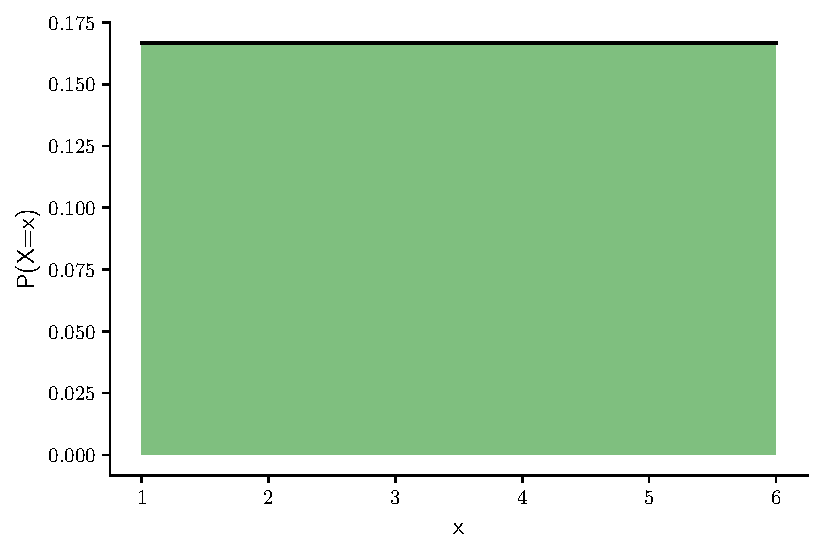
\includegraphics[width=0.5\linewidth]{./images/probabilitymassfunction_example.pdf}
		\caption{Probability Mass Function}
		\label{figure_probabilitymassfunction_example}
	\end{figure}

	Since the probability for all the random variables is same hence the graph is a flat line parallel to x-axis.
	
\end{tcolorbox}
\vfill
\pagebreak
\noindent
Now let us proceed with visualizing the probability density function
\\
\begin{tcolorbox}[colback=blue!5!white, colframe=blue!75!black, title = \textbf{Visualizing Probability Density Function}]
Let us visualize the data given in table \ref{table_probabilitydensityfunction_example}. Maximum individual have heights between 4.5 to 6 ft, this can be seen from the histogram in figure \ref{figure_probabilitydensityfunction_example}. Hence the probability for the same interval should also be highest. It can be observed from \ref{figure_probabilitydensityfunction_example} that probability for this interval is the highest 
	\begin{figure}[H]
		\centering
		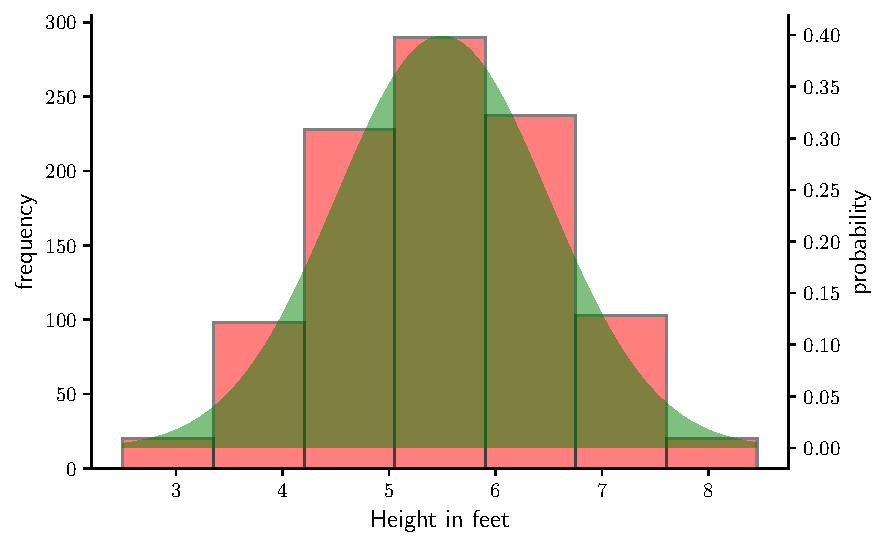
\includegraphics[width=0.5\linewidth]{./images/figure_probabilitydensityfunction_example.pdf}
		\caption{Probability Density Function}
		\label{figure_probabilitydensityfunction_example}
	\end{figure}

\end{tcolorbox}
\noindent
\\
Since now we are familiar with how to interpret the visual representation of Probability Mass Function and Probability Distribution Function, we will proceed further with cumulative distribution function
\\
\begin{tcolorbox}[colback=red!5!white, colframe=red!75!black, title = \textbf{Cumulative Distribution Function}]
	Cumulative Distribution Function for a random variable X is used to define the sum of probabilities for $ X \le x$ 
\end{tcolorbox}
\noindent
\\
If the random Variable X is discreet random variable then cumulative distribution function can be mathematically expressed as
$$ F(x) = P(X \le x) = \sum_{x_i}^{x} p(x) $$
\noindent
The cumulative distribution function of a discreet random variable X will have the following properties:
\begin{itemize}
	\item $ 0 \le F(x) \le 1 $
	\item $ \lim\limits_{x \rightarrow \infty} F = 1 $
	\item $ \lim\limits_{x \rightarrow -\infty} F = 0 $
	\item $a \textless b \rightarrow F(a) < F(b)$
\end{itemize}

\begin{tcolorbox}[colback=blue!5!white, colframe=blue!75!black, title = \textbf{Cumulative Distribution Function for Discreet Random Variable }] 
	Let us take an example of rolling of a dice, the probability of getting a number less than or equal to 1 is $\frac{1}{6}$, However the probability of getting a number less than or equal to 2 is $P(X \le 2) = p(1) + p(2) = \frac{1}{6} + \frac{1}{6} = \frac{2}{6}$
		\begin{table}[H]
		\centering
		\begin{tabular}{c|c}
			$\boldsymbol{X \le x}$ & $\boldsymbol{P(X \le x)}$      \\
			\hline
			$x \le 1$     & $\frac{1}{6}$ \\
			$x \le 2$     & $\frac{2}{6}$ \\
			$x \le 3$     & $\frac{3}{6}$ \\
			$x \le 4$     & $\frac{4}{6}$ \\
			$x \le 5$     & $\frac{5}{6}$ \\
			$x \le 6$     & $ 1 $
		\end{tabular}
		\caption{Cumulative Distribution Function for rolling of a dice}
	\end{table}

	\begin{figure}[H]
		\centering
			\begin{subfigure}[b]{0.3\textwidth}
				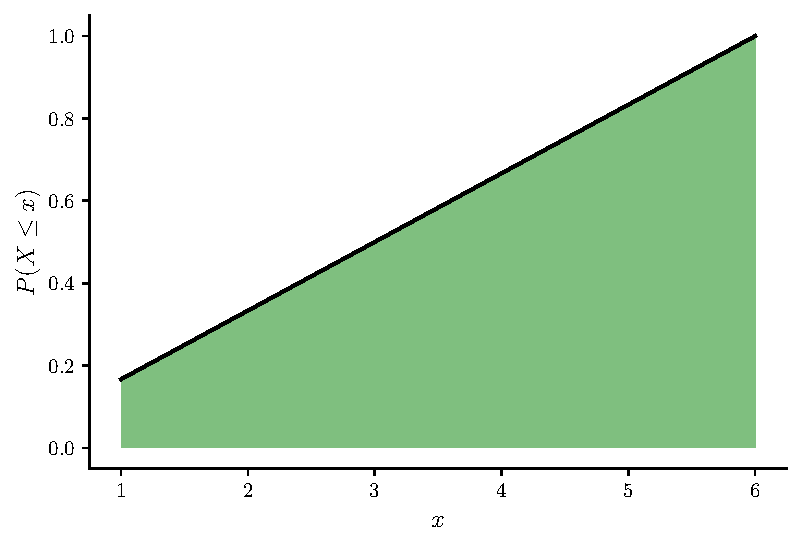
\includegraphics[width=\textwidth]{./images/cumulativedistributionfunction_dicrete_example.pdf}
		%		\subcaption{Univariate Line Graph}
			\end{subfigure}
			\begin{subfigure}[b]{0.3\textwidth}
				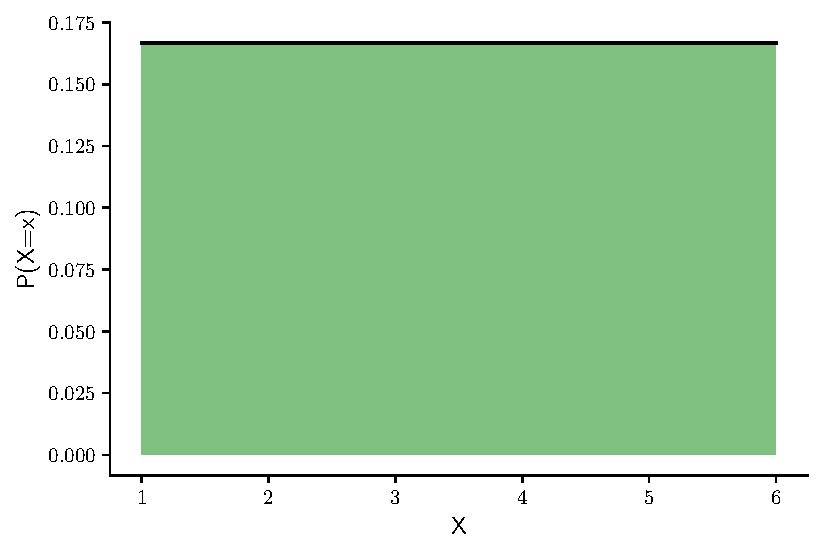
\includegraphics[width=\textwidth]{./images/figure_probabilitymassfunction_example.pdf}
		%		\subcaption{Multivariate Line Graph}
			\end{subfigure}
			\caption{Comparison of Cumulative Distribution Function and Probability Mass Function for rolling of a dice}
	\end{figure}

\end{tcolorbox}
\noindent
\\
If the cumulative distribution function represents a continuous random variable X, then the cumulative distribution function can be mathematically represented as
$$ F(x) = P(X \le x) = \int_{-\infty}^{x}f(x)dx $$
The cumulative distribution function of a continuous random variable X have the following characteristics:
\begin{itemize}
	\item $ 0 \le F(x) \le 1$
	\item $\lim\limits_{x \rightarrow \infty}F(x) = 1$
	\item $\lim\limits_{x \rightarrow -\infty}F(x) = 0 $
	\item $a < b \rightarrow F(a) \le F(b)$
\end{itemize} 
\vfill
\pagebreak
\begin{tcolorbox}[colback=blue!5!white, colframe=blue!75!black, title = \textbf{Cumulative Distribution Function for Probability Density Distribution}]
	For understanding this we will refer back to the example shown in figure \ref{figure_probabilitydensityfunction_example}. We can clearly see a peak in the center of the graph indicating that if an individual is selected at random the probability of this individual being 5 to 6 feet tall is highest. However cumulative distribution increases as height increases, this happens because of the addition of probability as the height increases.
	\\
	\\
	To understand it more intuitively, let us interpret it as follows, in our dataset the height of individuals range from 3 to 8 feet, the number of individuals who are very short i.e. around 3 ft and the number of individuals who are very tall i.e. around 8 feet are very less, hence there is very less probability that if an individual who is selected at random would be either very short or very tall. However when the concept of cumulative probability is applied to it the scenario changes. If we select the number of individuals who are less than or equal to 3 ft tall, then we cannot pick a lot of individuals as most of the people are taller than that i.e. cumulative frequency will be very less. However if we pick a the individuals who are more less than or equal to 8 ft tall, then this would include majority of people, hence the cumulative frequency will be high. This could be better visualized by figure \ref{cdf_comparison}   
	\begin{figure}[H]
		\centering
			\begin{subfigure}[b]{0.3\textwidth}
				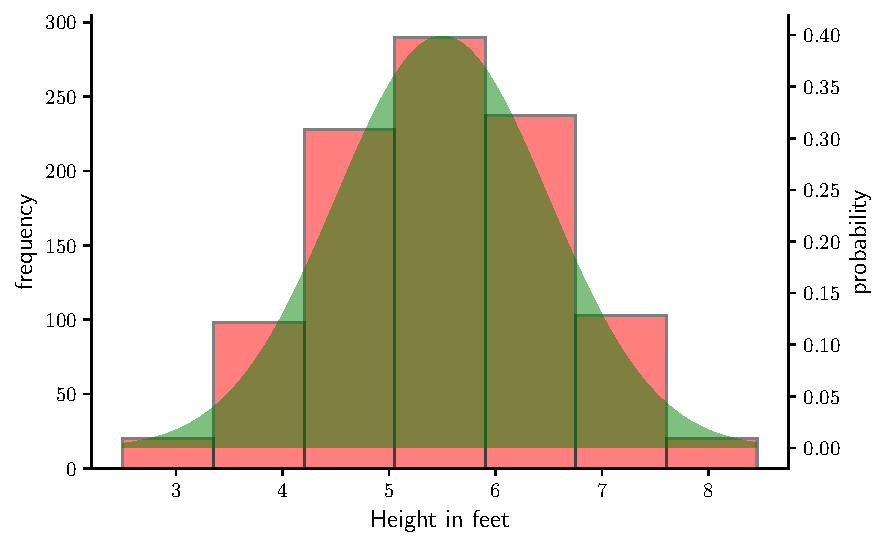
\includegraphics[width=\textwidth]{./images/figure_probabilitydensityfunction_example.pdf}
			\end{subfigure}
			\begin{subfigure}[b]{0.3\textwidth}
				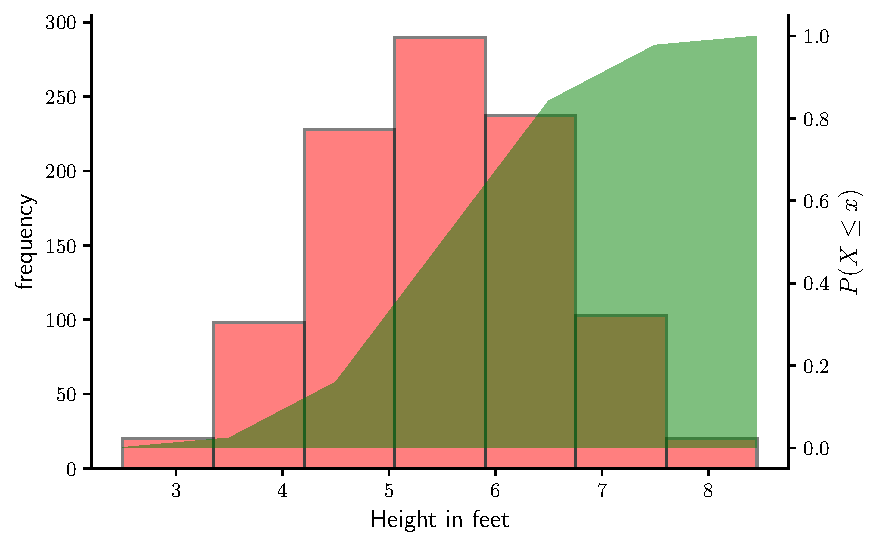
\includegraphics[width=\textwidth]{./images/figure_cumulativedistributionfunction_density_example.pdf}
			\end{subfigure}
		\caption{Comparison of Cumulative Distribution Function and Probability Density Function}
		\label{cdf_comparison}
	\end{figure}
	
\end{tcolorbox}

\section{Bernoulli Distribution Function}
In order to understand bernoulli distribution we first need to understand bernoulli trails
\\
\begin{tcolorbox}[colback=red!5!white, colframe=red!75!black, title = \textbf{Bernoulli Trial}]
	A Bernoulli Trial is an experiment with only one trial and two possible outcomes.  
\end{tcolorbox}
\noindent
\\
\textbf{Whenever we are dealing with the bernoulli distribution we either have the probability of a single event occuring or past data from repeated trials.}

\vfill
\pagebreak

While using the Bernoulli Distribution we often have to take the following into consideration:
\begin{itemize}
	\item Bernoulli Distribution has two outcomes $p$ and $1-p$
	\item The event with higher probability is considered to be $p$
	\item We often have to assign which outcome is 0 and which outcome is 1, usually the outcome with higher probability is assigned 1 and the other is assigned 0, i.e. $p$ is conventionally assigned $1$ and $1-p$ is assigned $0$ this makes sure that the expected outcome is $p$
\end{itemize} 

Thus based on the above we can say that for a bernoulli distribution
$$ \boxed{P(X=1) = p} $$
$$ \boxed{P(X=0) = 1-p} $$

Also
$$ \boxed{\sigma^{2} = p(1-p)} $$
$$ \boxed{\sigma = \sqrt{p(1-p)}} $$
$$ \boxed{\mu = p} $$
\\
Examples of a Bernoulli Trial include flipping of a coin
\\
\begin{tcolorbox}[colback=red!5!white, colframe=red!75!black, title = \textbf{Bernoulli Distribution Function}]
	Bernoulli Distribution Function is used to predict sucess i.e. $p$ or failure i.e. $q$ in a Bernoulli Trail
\end{tcolorbox}

\vfill
\pagebreak

\begin{tcolorbox}[colback=blue!5!white, colframe=blue!75!black, title = \textbf{Bernoulli Distribution Function}]
	Let us consider the flipping of a biased of coin, the weight distribution of the coin is such that it shows head 60 percent of the times. Calculate the probability of sucess and failure.
	\\
	\\
	It is given that
	$$ P(X=1) = p = 0.6 $$
	$$ P(X=0) = 1-p = 0.4 $$
	$$ \sigma^{2} = 0.6 \times 0.4 $$
	$$ \mu = 0.6 $$
	
	\begin{figure}[H]
		\centering
		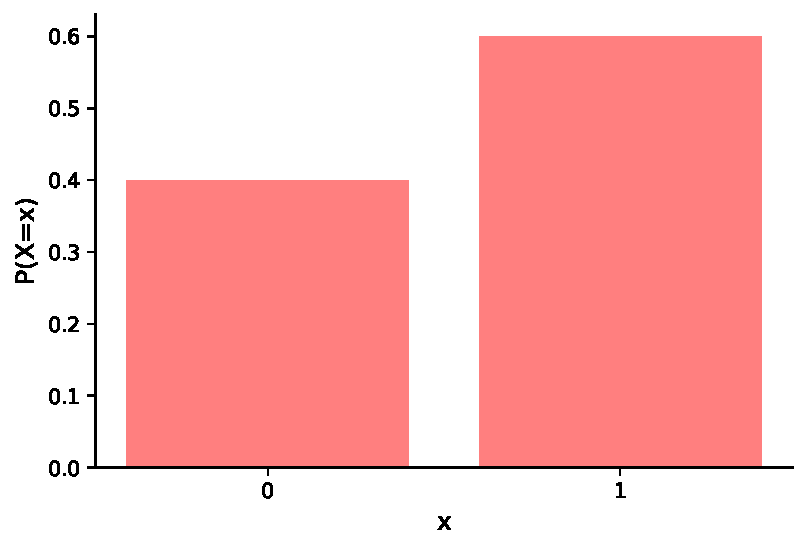
\includegraphics[width=0.5\linewidth]{./images/bernoulli_example.pdf}
		\caption{Bernoulli Distribution}
		\label{figure_bernoulli_example}
	\end{figure}

\end{tcolorbox}

\section{Binomial Distribution Function}

\begin{tcolorbox}[colback=red!5!white, colframe=red!75!black, title = \textbf{Binomial Distribution Function}]
	Binomial Distribution Function is a probability mass function used to calculate the probability of occurrence of an event exactly $x$ number of times in $n$ attempts. If $p$ is the probability of outcome $y$ in a single independent trial then binomial probability function can be given as
	$$ \boxed{P(X=x) = C^{n}_{x} p^{x} (1-p)^{n-x}} $$  
\end{tcolorbox}
\noindent
\\
Variance, standard deviation and mean can be calculated as
$$ \boxed{\sigma^{2}=np(1-p)} $$
$$ \boxed{\sigma = \sqrt{np(1-p)}} $$
$$ \boxed{\mu = np} $$

\vfill
\pagebreak

\begin{tcolorbox}[colback=blue!5!white, colframe=blue!75!black, title = \textbf{Binomial Distribution Function}]
	Let us consider a factory manufactures one car every minute and there is a 40 percent chance that the car produced will be defective. What is the probability that the factory will make 3 defective cars in next 5 minutes ? 
	\\
	\\
	Here we have,
	$$ x=3 $$
	$$ n=5 $$
	$$ p=0.4 $$
	Thus 
	$$P(X=3) = C^{5}_{3} 0.4^{3}(1-0.4)^{5-3}$$
	$$ P(X=3) = \frac{5!}{3!(5-3)!} 0.4^{3}(1-0.4)^{5-3} $$
	$$ P(X=3) = \frac{5 \times 4 \times 3!}{3!2!} 0.4^{3} 0.6^{2} $$	
	$$ P(X=3) = 10 \times 0.064 \times 0.36 $$
	$$ P(X=3) = 0.2304 $$
	
	Thus there is a 23.04 percent chance that the next 3 out of 5 cars will be defective 
	
	\begin{figure}[H]
		\centering
		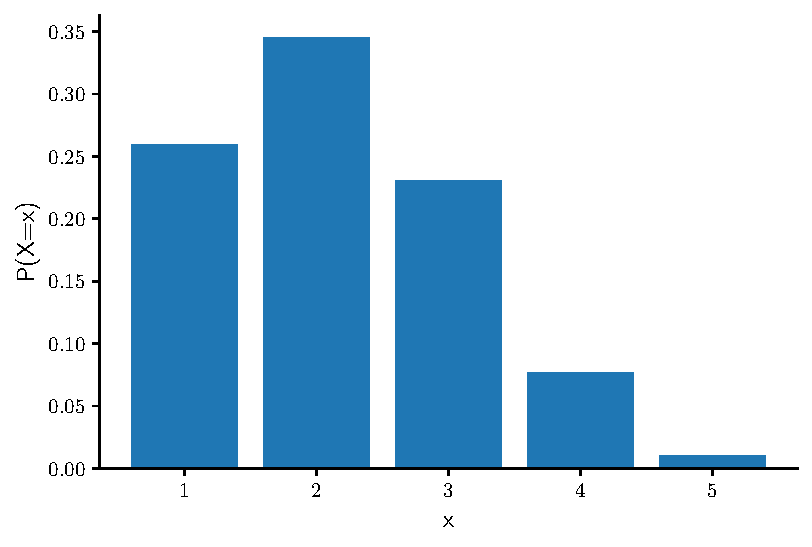
\includegraphics[width=0.5\linewidth]{./images/binomial_example.pdf}
		\caption{Binomial Distribution}
		\label{figure_binomial_example}
	\end{figure}

\end{tcolorbox}
\noindent
\\

\begin{figure}[H]
	\centering
	\begin{subfigure}[b]{0.3\textwidth}
		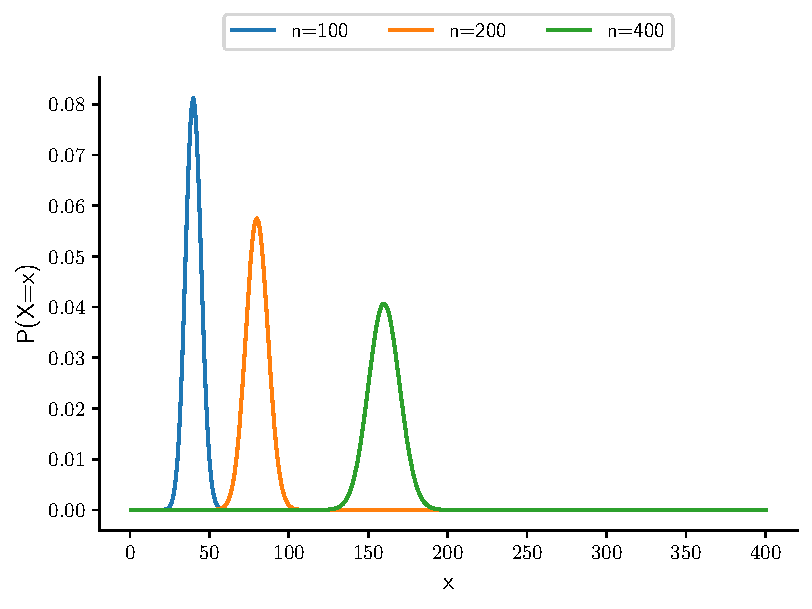
\includegraphics[width=\textwidth]{./images/binomial_example_n.pdf}
		\subcaption{Binomial Probability Distribution for different values of n}
	\end{subfigure}
	\begin{subfigure}[b]{0.3\textwidth}
		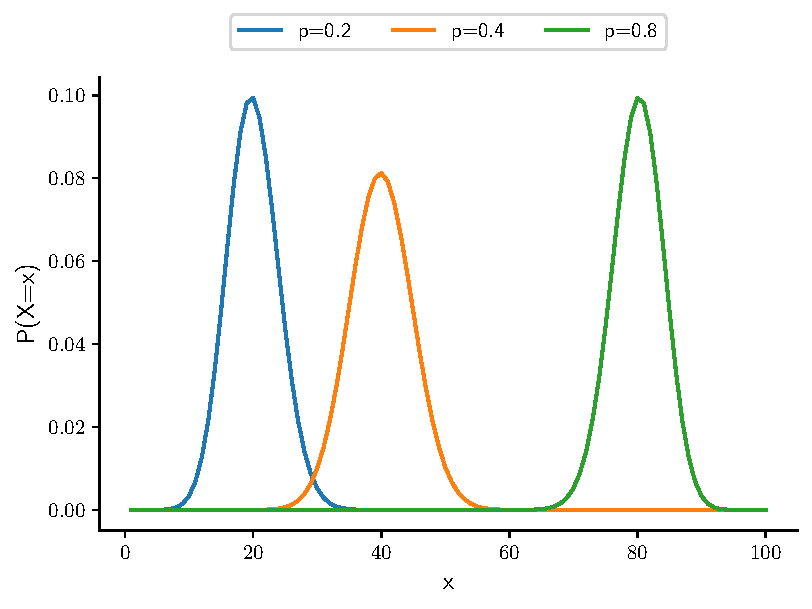
\includegraphics[width=\textwidth]{./images/binomial_example_p.pdf}
		\subcaption{Binomial Probability Distribution for different values of p}
	\end{subfigure}
	\caption{Comparison of Binomial Probability Distribution with varying parameters}
	\label{figure_binomial_comparison}
\end{figure}
\noindent
The formulae for binomial probability distribution depends on
\begin{itemize}
	\item $n$
	\item $p$
	\item $x$
\end{itemize}
\noindent
However the probability distribution is not affected by $x$. Binomial Distribution shows significant variation for different values of $p$ and $n$. As the value of $n$ increases for a given value of $p$ the peak of the curve shifts towards right but decreases in height. It must be noted that peak of the curve is always at the mean of the distribution.
\\
\\
For a fixed value of $n$ the peak of the curve shifts towards right as the value of $p$ increases. However the height of the peak follows no significant pattern.
\\
\\
\textbf{Thus we can say that the for Binomial Probability Distribution the peak of the curve always coincides with the mean of the distribution}  


\section{Poisson Distribution Function}

\begin{tcolorbox}[colback=red!5!white, colframe=red!75!black, title = \textbf{Poisson Distribution Function}]
	Poisson Distribution is a Probability Mass Function used to predict the probability of specific number of occurrences of an event in a given time frame, distance or length by using the frequency of occurrence of that event $\lambda$ from previous observations. If an event occurs $\lambda$ times in a unit distance, time or length then the probability of that event occurring $x$ times in another unit of time, length or distance can be given as
	$$ \boxed{P(X=x) = \frac{e^{-\lambda} \lambda^{x}}{x!}} $$

\end{tcolorbox}
\noindent
\\
The mean and standard deviation of the distribution is given as
$$ \boxed{\mu = \lambda} $$
$$ \boxed{\sigma = \sqrt{\mu}} $$

\begin{tcolorbox}[colback=blue!5!white, colframe=blue!75!black, title = \textbf{Poisson Distribution Function}]
	If 10 customers arrive at billing counter of a supermarket in an hour, what is the probability that 15 customers would come at the billing counter in the next 1 hour?
	\\
	\\
	Here we know
	$$ \lambda = 10 $$
	$$ x = 15 $$
	Therefore
	$$ P(X=15) = \frac{2.718^{-10} 10^{15}}{15!} $$
	$$ P(X=15) = 0.03472 $$	
	
	\begin{figure}[H]
		\centering
		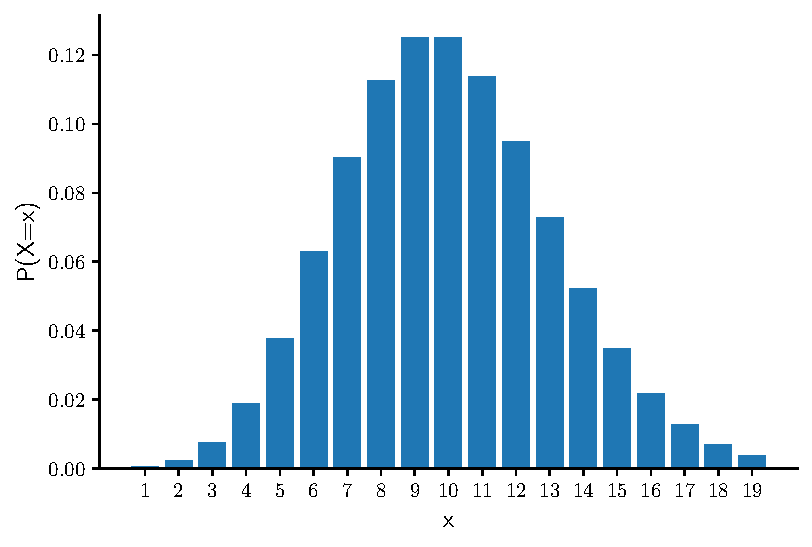
\includegraphics[width=0.5\linewidth]{./images/poission_example.pdf}
		\caption{Poisson Distribution}
		\label{figure_poission_example}
	\end{figure}

\end{tcolorbox}

\vfill
\pagebreak

\begin{figure}[H]
	\centering
	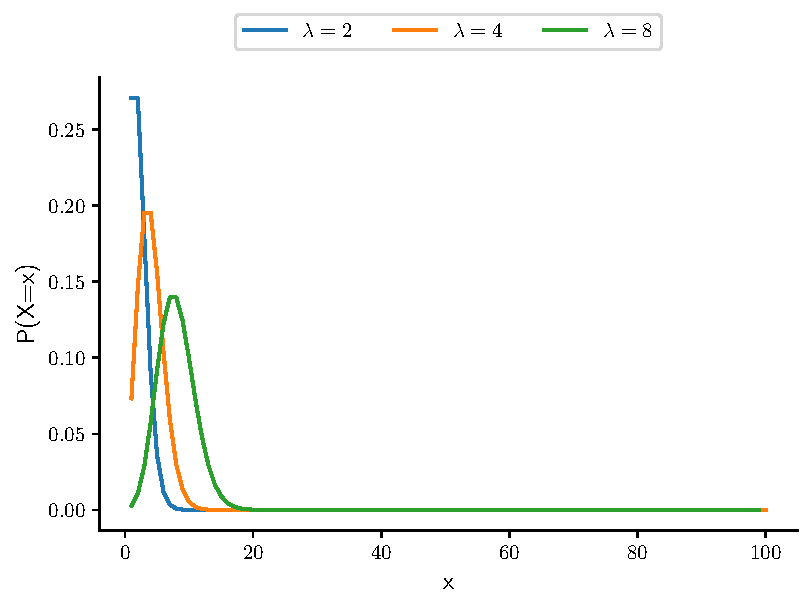
\includegraphics[width=0.5\linewidth]{./images/poission_example_u.pdf}
	\caption{Poisson Distribution Function for different values of $\lambda$}
	\label{figure_poission_example_u}
\end{figure}
\noindent
As we can see from figure \ref{figure_poission_example_u} probability distribution for Poisson Distribution Function depends on $\lambda$. As the value of $\lambda$ increases the peak of the curve shifts towards right and becomes smaller.

\section{Exponential Distribution Function}

Exponential Distribution Function can be seen as inverse of Poisson Distribution Function. Poisson Distribution uses the number of events per unit time,length or distance where as exponential distribution is used to predict the time between two consecutive events. For example Poisson Distribution looks at number of people arriving at a billing counter in one hour where as exponential distribution will look at  the time between two consecutive arrivals of costumer. 
\\
\begin{tcolorbox}[colback=red!5!white, colframe=red!75!black, title = \textbf{Exponential Probability Distribution}]
	Exponential Distribution Function is a probability density function used to calculate the probability of time between events. It can be mathematically expressed as
	$$ \boxed{P(X = x) = \frac{e^{\frac{-x}{\mu}}}{\mu}}$$
	where
	$$ \boxed{\mu = \frac{1}{\lambda}} $$
\end{tcolorbox}
\noindent
\\
For a distribution to be classified as exponential probability distribution, the following must be true:
\begin{itemize}
	\item Events must occur at a constant rate
	\item Events must be independent of each other.
\end{itemize}

\noindent
The mean and variance of Exponential distribution function can be calculated as follows
$$\boxed{\mu = \frac{1}{\lambda}} $$
$$\boxed{\sigma^2 = \frac{1}{\lambda^2}}$$
\noindent
The Cumulative Distribution Function for Exponential Probability Distribution is given as
$$\boxed{P(X < x) = 1 - e^{\frac{-x}{\mu}}} $$ 

\vfill
\pagebreak

\noindent
Any Piosson Distribution can be converted to exponential distribution as follows
\\
\begin{tcolorbox}[colback=blue!5!white, colframe=blue!75!black, title = \textbf{Exponential Distribution Function}]
	Let us consider 6 unique visitors arrive at an e-commerce website every minute. What is the probability that another visitor is gonna arrive in
	\begin{itemize}
		\item within next 5 seconds
		\item after 10 second
		\item exactly at 15 seconds
	\end{itemize}
	Here 
	$$ \lambda = 6 \mbox{ per minute} $$
	Therefore
	$$ \mu = \frac{1}{6}\mbox{ minute} = 10 \mbox{ seconds} $$
	
	Thus
	$$ P(X < 5) =  1 - e^{\frac{-5}{20}} = 0.393$$
	
	Similarly
	$$ P(X > 10) =  1- (1 - e^{\frac{-10}{20}}) $$
	$$ P(X > 10) =  e^{\frac{-10}{20}} = 0.607$$
	$$ P(X = 15) =  \frac{e^{\frac{-15}{10}}}{10} = 0.022 $$
	
	\begin{figure}[H]
		\centering
		\begin{subfigure}[b]{0.3\textwidth}
			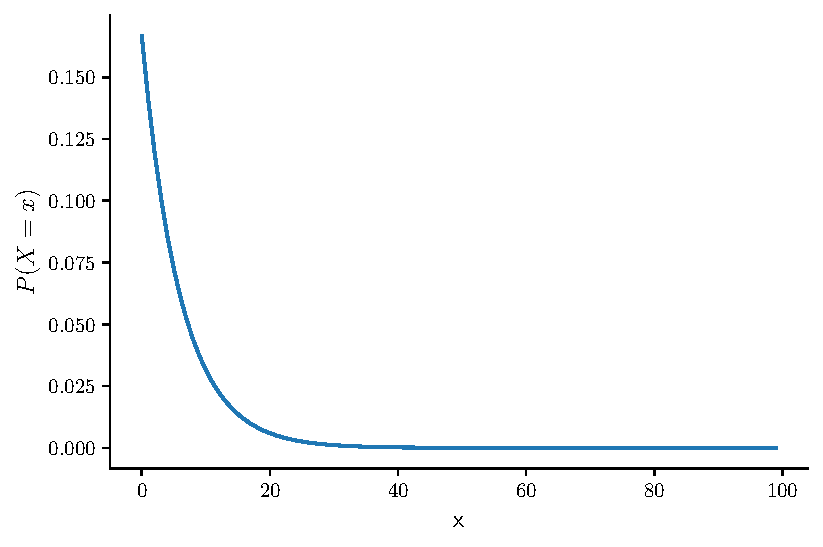
\includegraphics[width=\textwidth]{./images/exponentail_example.pdf}
			\subcaption{Probability Density Function for Exponential Distribution}
		\end{subfigure}
		\begin{subfigure}[b]{0.3\textwidth}
			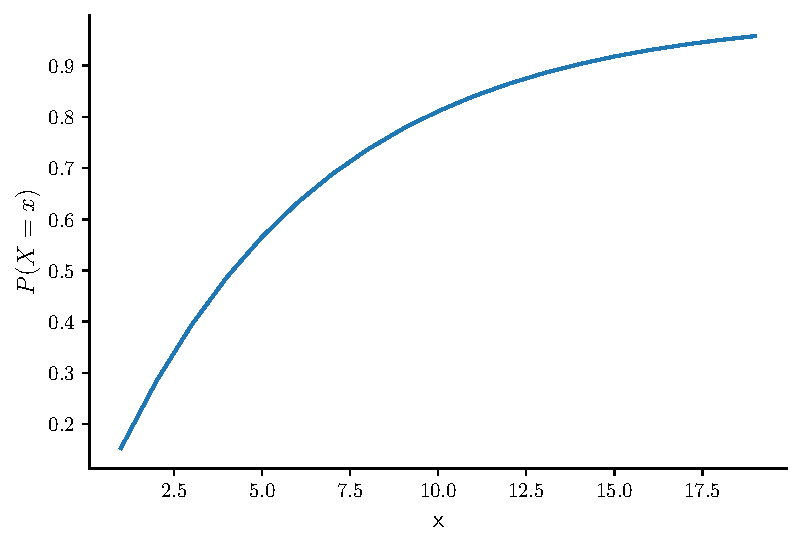
\includegraphics[width=\textwidth]{./images/exponentail_example_cdf.pdf}
			\subcaption{Cumulative Distribution Function for Exponential Distribution}
		\end{subfigure}
		\caption{Probability Density Function and Cumulative Distribution Function for Exponential Distribution}
		\label{figure_exponentail_example}
	\end{figure}
	
\end{tcolorbox}

\vfill
\pagebreak

\begin{figure}[H]
	\centering
	\begin{subfigure}[b]{0.3\textwidth}
		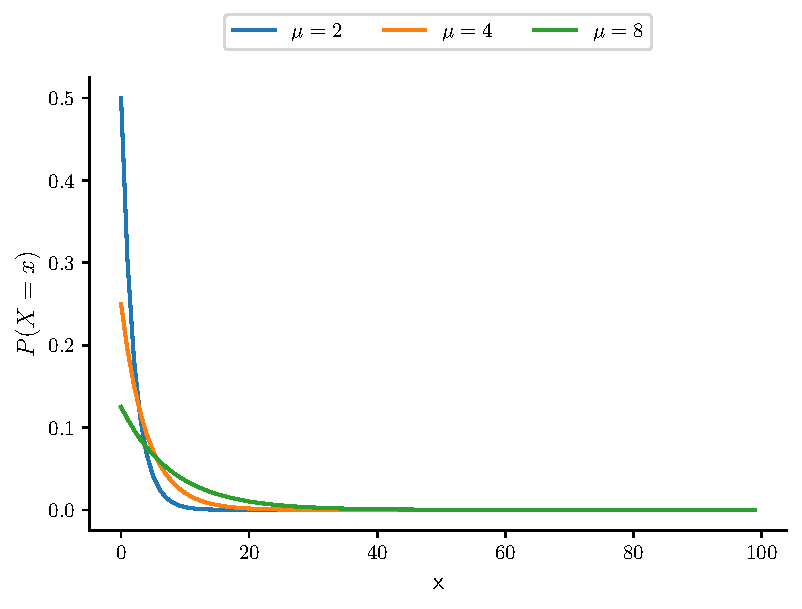
\includegraphics[width=\textwidth]{./images/exponentail_example_mu.pdf}
		\subcaption{Effect of $\mu$ on PDF for Exponential PRobability Distribution}
	\end{subfigure}
	\begin{subfigure}[b]{0.3\textwidth}
		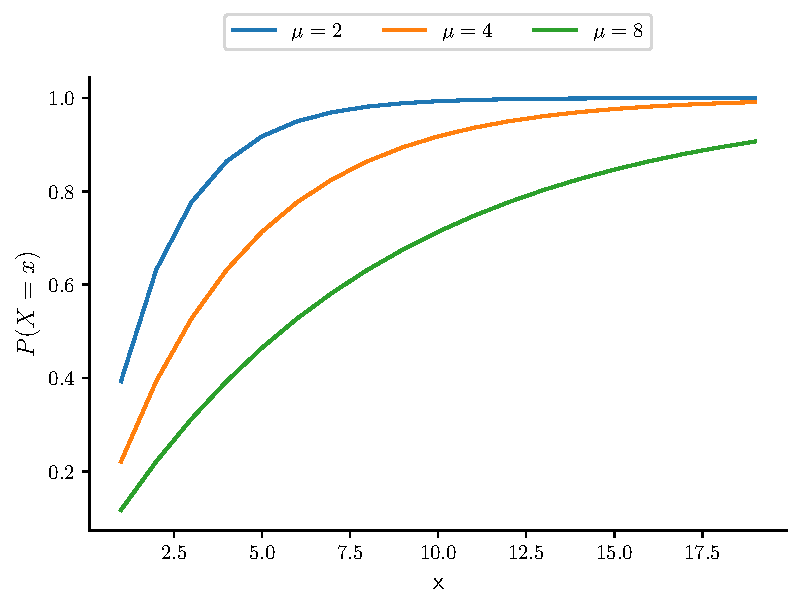
\includegraphics[width=\textwidth]{./images/exponentail_example_cdf_mu.pdf}
		\subcaption{Effect of $\mu$ on CDF for Exponential PRobability Distribution}
	\end{subfigure}
	\caption{Probability Density Function and Cumulative Distribution Function for Exponential Distribution}
	\label{figure_exponentail_example_mu}
\end{figure}
\noindent
As can be seen from figure \ref{figure_exponentail_example_mu} that value of $\mu$ affects the probability distribution for both PDF and CDF of exponential function. As the value of $\mu$ increases the maximum probability of the event decreases. But this is not true for CDF, as the value of $\mu$ decreases the cumulative distribution tends to take a higher value for higher values of $x$.  

\section{Geometric Distribution Function}

\begin{tcolorbox}[colback=red!5!white, colframe=red!75!black, title = \textbf{Geometric Distribution}]
	Geometric Distribution Function is a Probability Mass Function used to calculate that your first success will be on the $n^{th}$ try. It can be mathematically expressed as
	$$\boxed{P(X = x) = (q)^{x-1}p} $$ 
\end{tcolorbox}
\noindent
\\
The mean and variance of Geometric Distribution Function are given as
$$ \boxed{\mu =  \frac{1-p}{p}}$$
$$\boxed{\sigma^2 = \frac{1-p}{p^2}}$$
Let us elaborate with an example
\\
\begin{tcolorbox}[colback=blue!5!white, colframe=blue!75!black, title = \textbf{Geometric Distribution}]
	Let us consider that the probability of a basketball player making a successful free throw is 20 \%. What is the probability that the first successful free throw will be after 10 failed trials ?
	\\
	We have
	$$ p = \frac{20}{100} $$
	$$ q = 1 - \frac{20}{100} = \frac{80}{100}$$
	Thus
	$$ P(X = 10) = (0.8)^{10-1} \times 0.2 $$
	$$ P(X = 10) = 0.027 $$
	
	\begin{figure}[H]
		\centering
		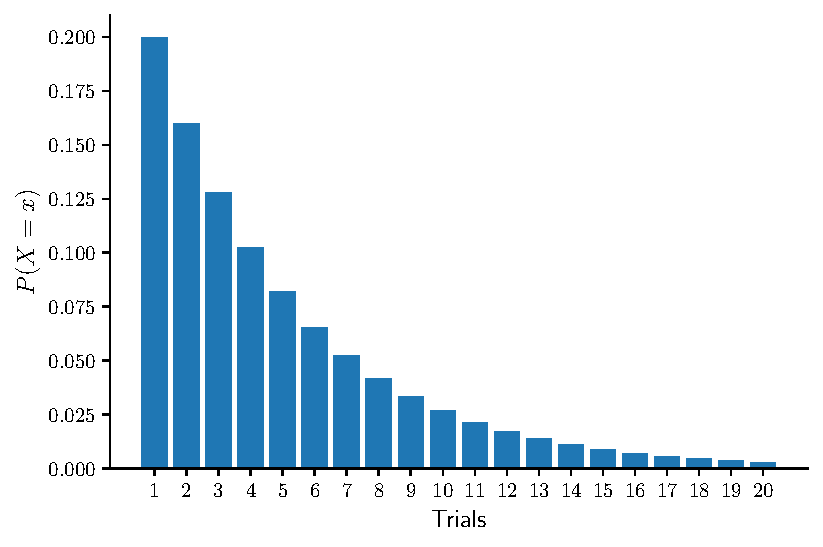
\includegraphics[width=0.5\linewidth]{./images/geometric_example.pdf}
		\caption{Geometric Distribution}
		\label{figure_geometric_example}
	\end{figure}
	
\end{tcolorbox}
\noindent
\\
\begin{figure}[H]
	\centering
	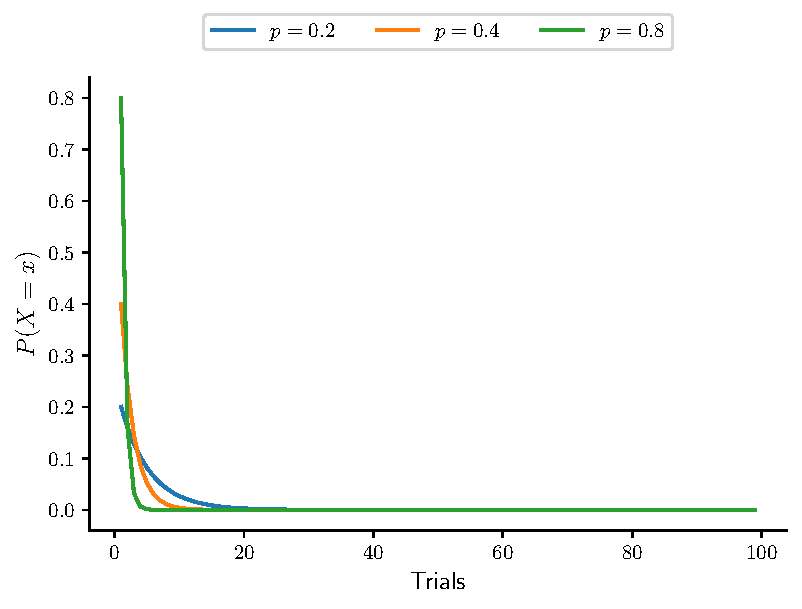
\includegraphics[width=0.5\linewidth]{./images/geometric_example_p.pdf}
	\caption{Geometric Distribution}
	\label{figure_geometric_example_p}
\end{figure}
\noindent
The effect of probability of success on Geometric Probability Distribution can be seen in figure \ref{figure_geometric_example_p}.

\section{Negative Binomial Distribution Function}

\begin{tcolorbox}[colback=red!5!white, colframe=red!75!black, title = \textbf{Negative Binomial Distribution}]
	Negative Binomial Function is a Probability Mass Function used to calculate the number of trials($k$) required to get $x^{th}$ success.
	$$ \boxed{P(X=x) = C^{x-1}_{k-1}p^{k} (1-p)^{k-x}} $$
\end{tcolorbox}
\noindent
\\
Let us illustrate with an example.
\\\begin{tcolorbox}[colback=blue!5!white, colframe=blue!75!black, title = \textbf{Negative Binomial Distribution}]
	If a basketball player makes 3 successful free throws for every 5 attempts, what is the probability that $7^{th}$ successful free throw will be made in the $13^{th}$ attempt ?
	\\
	\\
	We have
	$$ p = \frac{3}{5} $$
	$$ x = 7 $$
	$$ k = 13 $$
	$$ P(X = 13) = \frac{(13-1)!}{(7-1)!(13-7)!} \times \left(\frac{3}{5}\right)^{7} \times \left( 1-\frac{3}{5} \right) ^ {13-7} $$
	$$ \frac{12!}{6! \times 6!} \times \left(\frac{3}{5}\right)^{7} \times \left( \frac{2}{5} \right) ^ 6 = 0.005 $$
\end{tcolorbox}

\section{Normal Distribution Function}

As we did in a previous section, here also we will refrain from providing a formal definition and will focus more on the idea of Normal Distribution. 
\\
\\
Normal Distribution can be seen in many spectrum of life. Before we explore these examples let us briefly look at what is normal distribution.
\\
\\
Normal Distribution is a type of Probability Density Function. If a random variable is normally distributed than the data points will cluster around the mean i.e. most of the values will be close to the mean and as we move away from the mean the frequency of values will decrease. As shown in figure \ref{figure_normal_example}.
\\
\\
\begin{figure}[H]
	\centering
	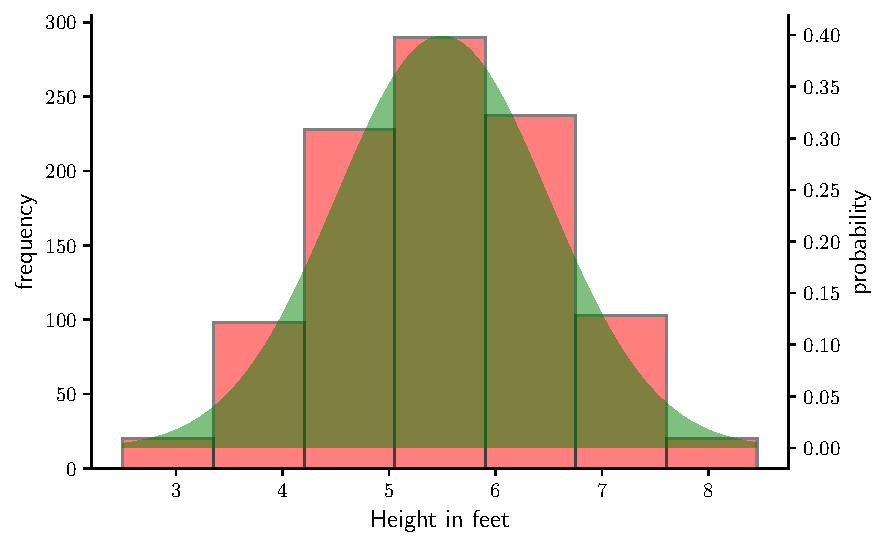
\includegraphics[width=0.5\linewidth]{./images/figure_probabilitydensityfunction_example.pdf}
	\caption{Normal Distribution}
	\label{figure_normal_example}
\end{figure}
\noindent
If we closely observe figure \ref{figure_normal_example} we can observe that it is a distribution plot and an area graph. The mean of the distribution is 5.5 and most of the values lie in the same interval as that of mean hence we can observe that the height of the graph is highest since most of the values lie in the same interval as that of the mean thus if a value is picked at random the probability that it will lie in the same interval as that of the mean is highest, hence we can see that the probability curve peaks out at the mean.  
\\
\\
In a normal distribution the probability of random variable $X$ being equal to $x$ can be calculated as
$$ \boxed{P(X = x) = \frac{1}{\sigma \sqrt{2 \pi}}e^{\frac{{-(x - \mu)^2}}{2 {\sigma}^2}} }$$
\noindent
The above equation will give the area to the left of the curve for a given value of $x$.
\\
\begin{tcolorbox}[colback=blue!5!white, colframe=blue!75!black, title = \textbf{Normal Distribution}]
	If the heights of a group of individuals is normally distributed with a mean of 5.5 feet and standard deviation of 0.5 feet, what is the probability that an individual selected at random will have a height of 4.5 feet?
	\\
	\\
	We know tha
	$$ \mu = 5.5 $$
	$$ \sigma = 0.5 $$
	$$ P(X = 4.5) = \frac{1}{0.5 \times \sqrt{2 \pi}} e^{\frac{-(4.5 - 5.5)^2}{2 \times (0.5)^2}}  = 0.107 $$ 
\end{tcolorbox}
\noindent
\\
As can be seen from above equation, the probability of random variable $X$ in normally distributed data depends on $\sigma$ and $\mu$.

\subsection{Effect of standard deviation and mean}

\begin{figure}[H]
	\centering
	\begin{subfigure}[b]{0.3\textwidth}
		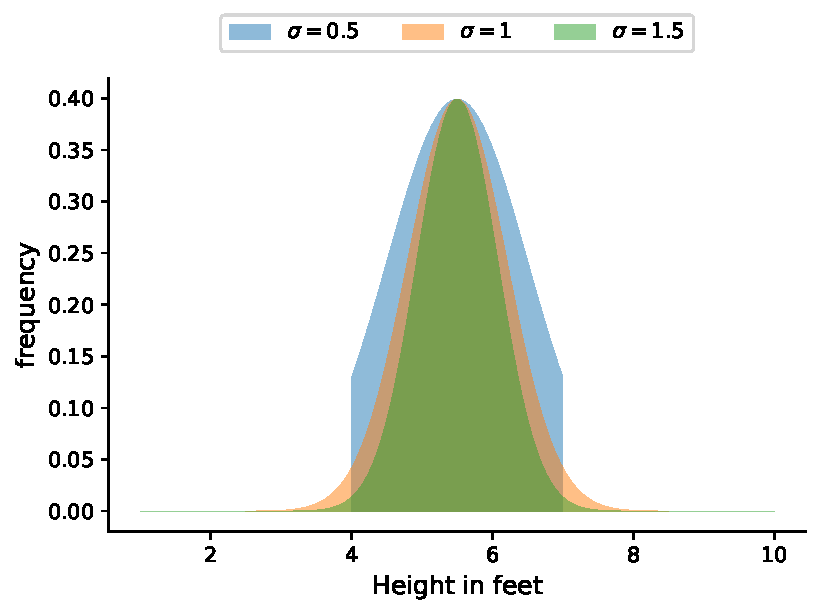
\includegraphics[width=\textwidth]{./images/normal_example_d.pdf}
		\subcaption{Effect of $\sigma$ on Normal Probability Distribution}
	\end{subfigure}
	\begin{subfigure}[b]{0.3\textwidth}
		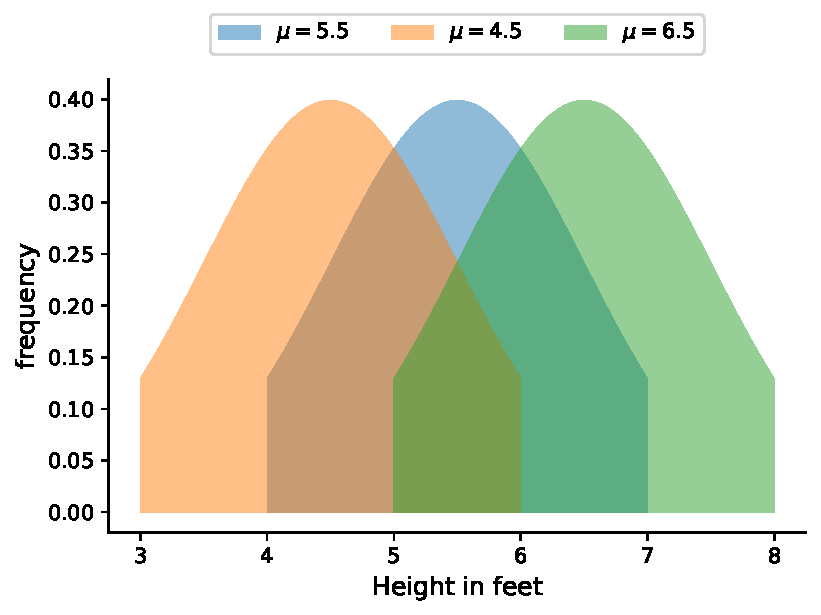
\includegraphics[width=\textwidth]{./images/normal_example_m.pdf}
		\subcaption{Effect of $\mu$ on Exponential Probability Distribution}
	\end{subfigure}
	\caption{Effect of $\mu$ and $\sigma$ on Normal Probability Distribution}
	\label{figure_normal_example_d_mu}
\end{figure}

As discussed above, the mean and standard deviation are the two driving factors in normal distribution. As mentioned above, in a normal distribution the data clusters around the mean, hence if we change the mean the peak of the bell curve will shift accordingly.
\\
\\
The mean of the distribution determines the location of the peak of the curve. Similarly Shape of the bell curve is determined by the standard deviation. The higher the value of standard deviation the more widespread will be the shape of the curve.
\\
\subsection{Skewness and Kurtosis}

As can be seen in figure \ref{figure_normal_example_d_mu}, the normal distribution is symmetrically distributed around the mean. But this is not always the case. may times the values tend to cluster towards one end of the spectrum. This clustering of values is what is known as skew.

\begin{figure}[H]
	\centering
	\begin{subfigure}[b]{0.3\textwidth}
		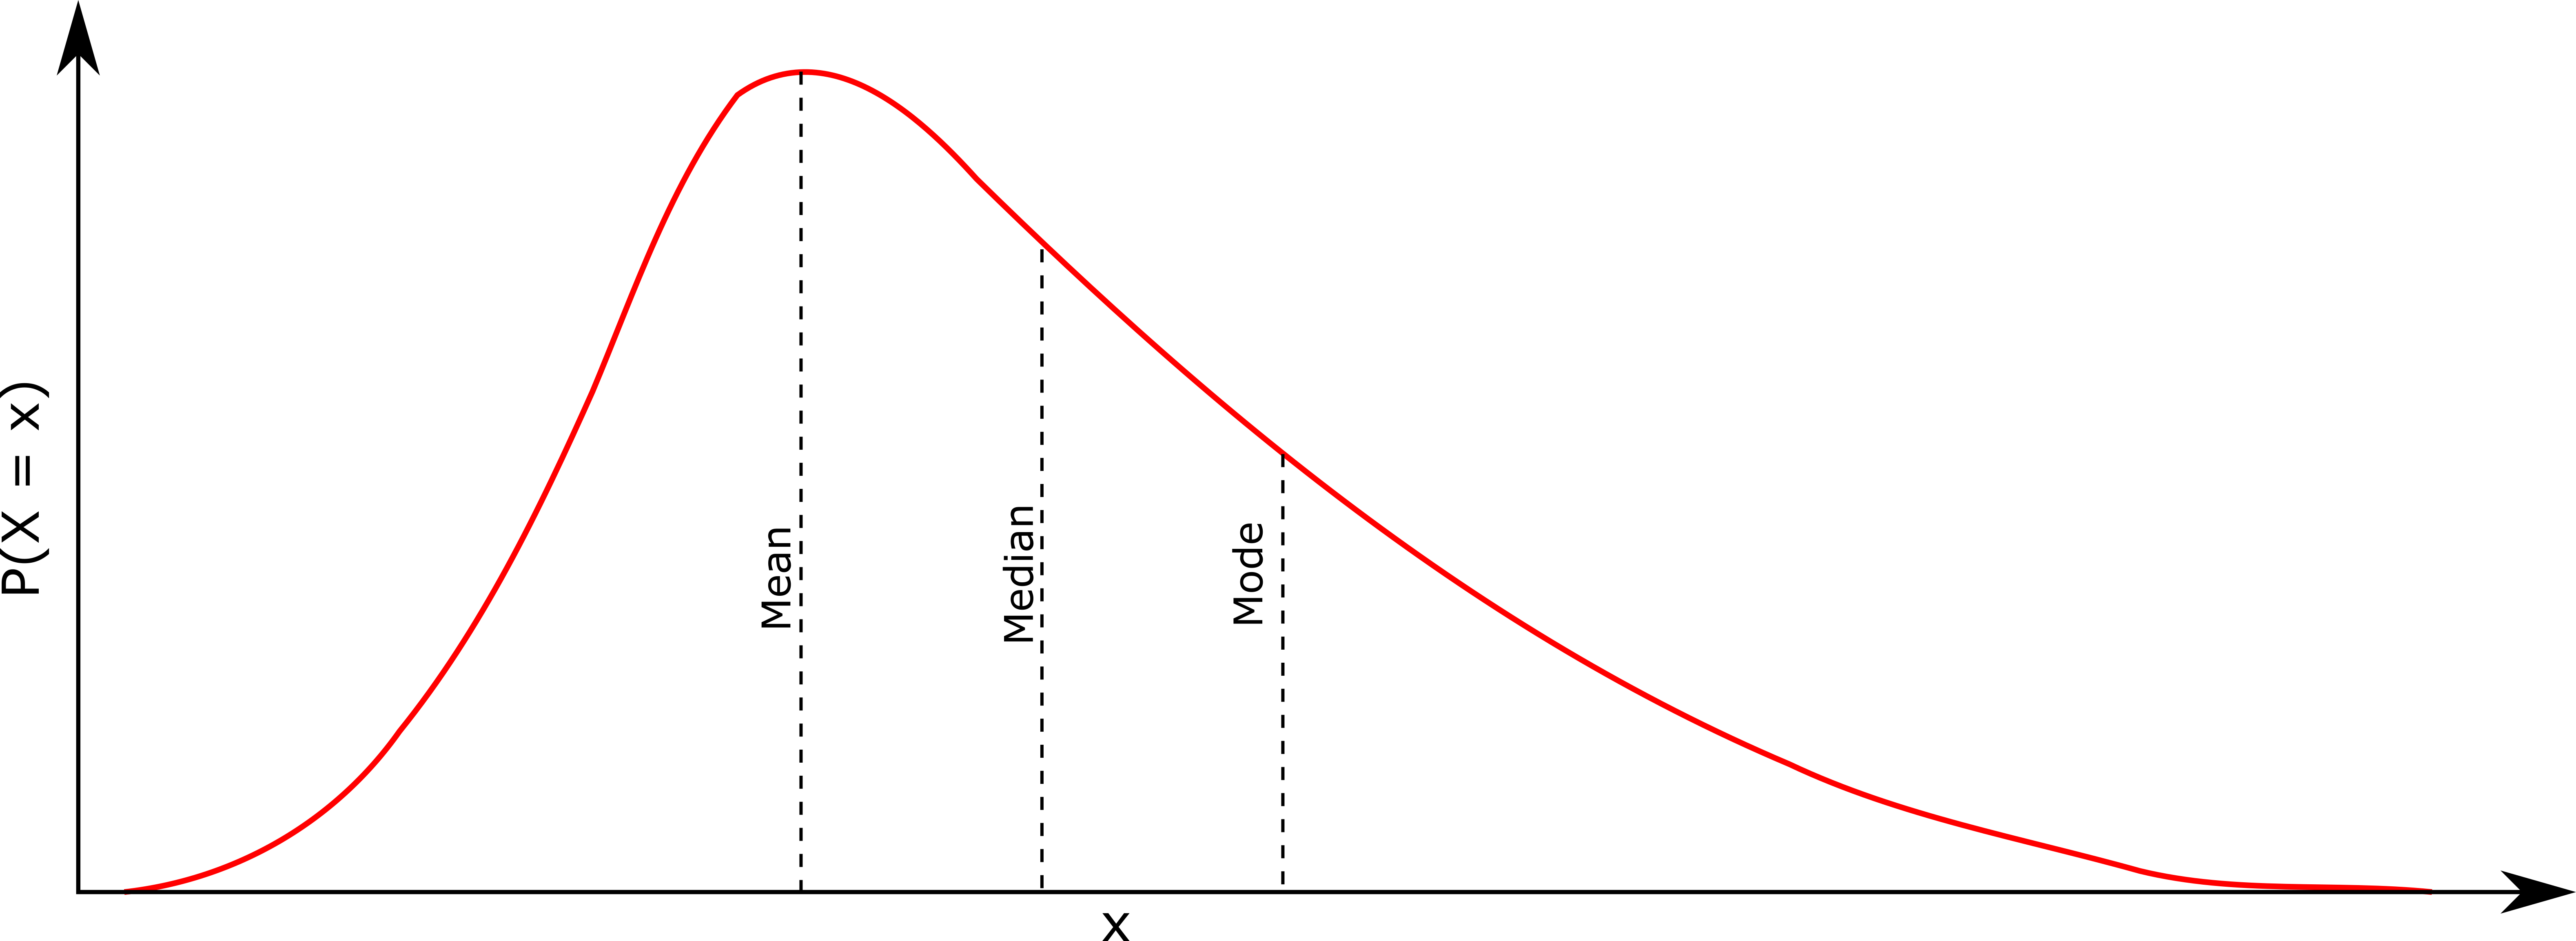
\includegraphics[width=\textwidth]{./images/normal_left.png}
		\subcaption{Right Skewed(Positive Skew) Normal Distribution Curve}
	\end{subfigure}
	\begin{subfigure}[b]{0.3\textwidth}
		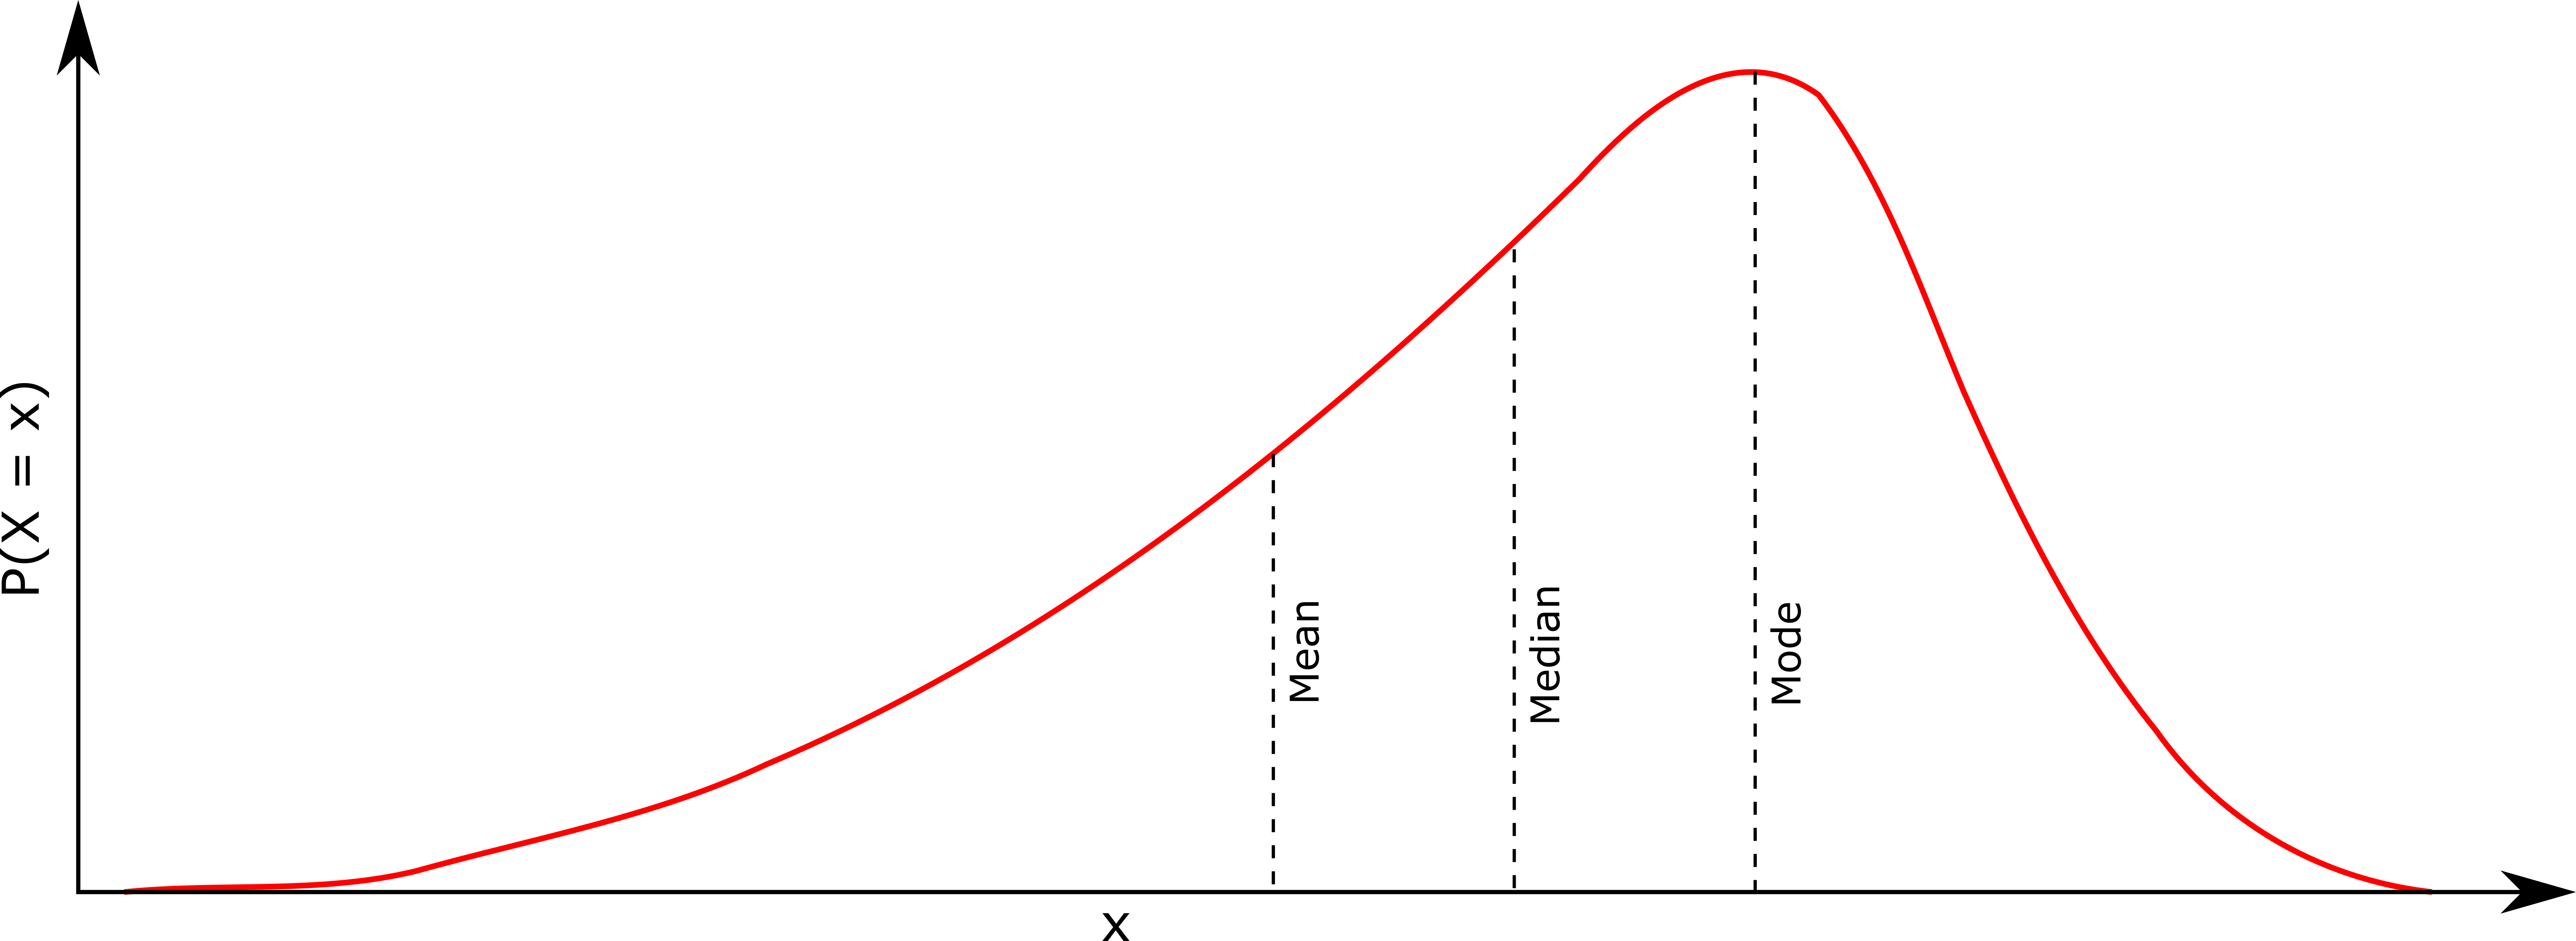
\includegraphics[width=\textwidth]{./images/normal_right.png}
		\subcaption{Left Skewed(Negitive Skew) Normal Distribution Curve}
	\end{subfigure}
	\caption{Skewness in Normal Distribution Curve}
\end{figure}
\noindent
In a normal distribution the data is equally clustered around the mean i.e. there are equal number of observation which are either smaller or larger than mean.
\\
\\
\textbf{If the number of observations greater than the mean have a higher frequency than the number of observation smaller than the mean, the data is said to be Right Skewewd or Positively Skewed.}
\\
\\
If the data is positively skewed than the mean, median and mode will have the following relationship
$$ mean < median < mode $$
\\
\\
\textbf{If the number of observations smaller than the mean have a higher frequency than the number of observation greater than the mean, the data is said to be Left Skewed or Negatively Skewed.}
\\
\\
For a left skewed data the following is true
$$ mean > median > mode $$
\\
If the data is skewed than there is a sepration between mean median and mode. This sepration has been made the basis of skewness calculation however now a moment based approach is followed based on the method of moments. MEthod of moments is not the focus of this chapter, hence we will not go deeper in to the method of moments.
\\
\\
Based on the method of moments, skewness for population can be calculated as 
$$\boxed{skew_{sample} = \frac{n}{(n-1)(n-2)} \frac{\sum (x - \bar{x})^3}{s^{3}}} $$
\\
\\
The formulae for population skewness can be given as
$$ \boxed{skew_{population} = \frac{1}{n} \frac{\sum (x - \mu)^3}{\sigma^3}} $$
\\
\\
\begin{figure}[H]
	\centering
	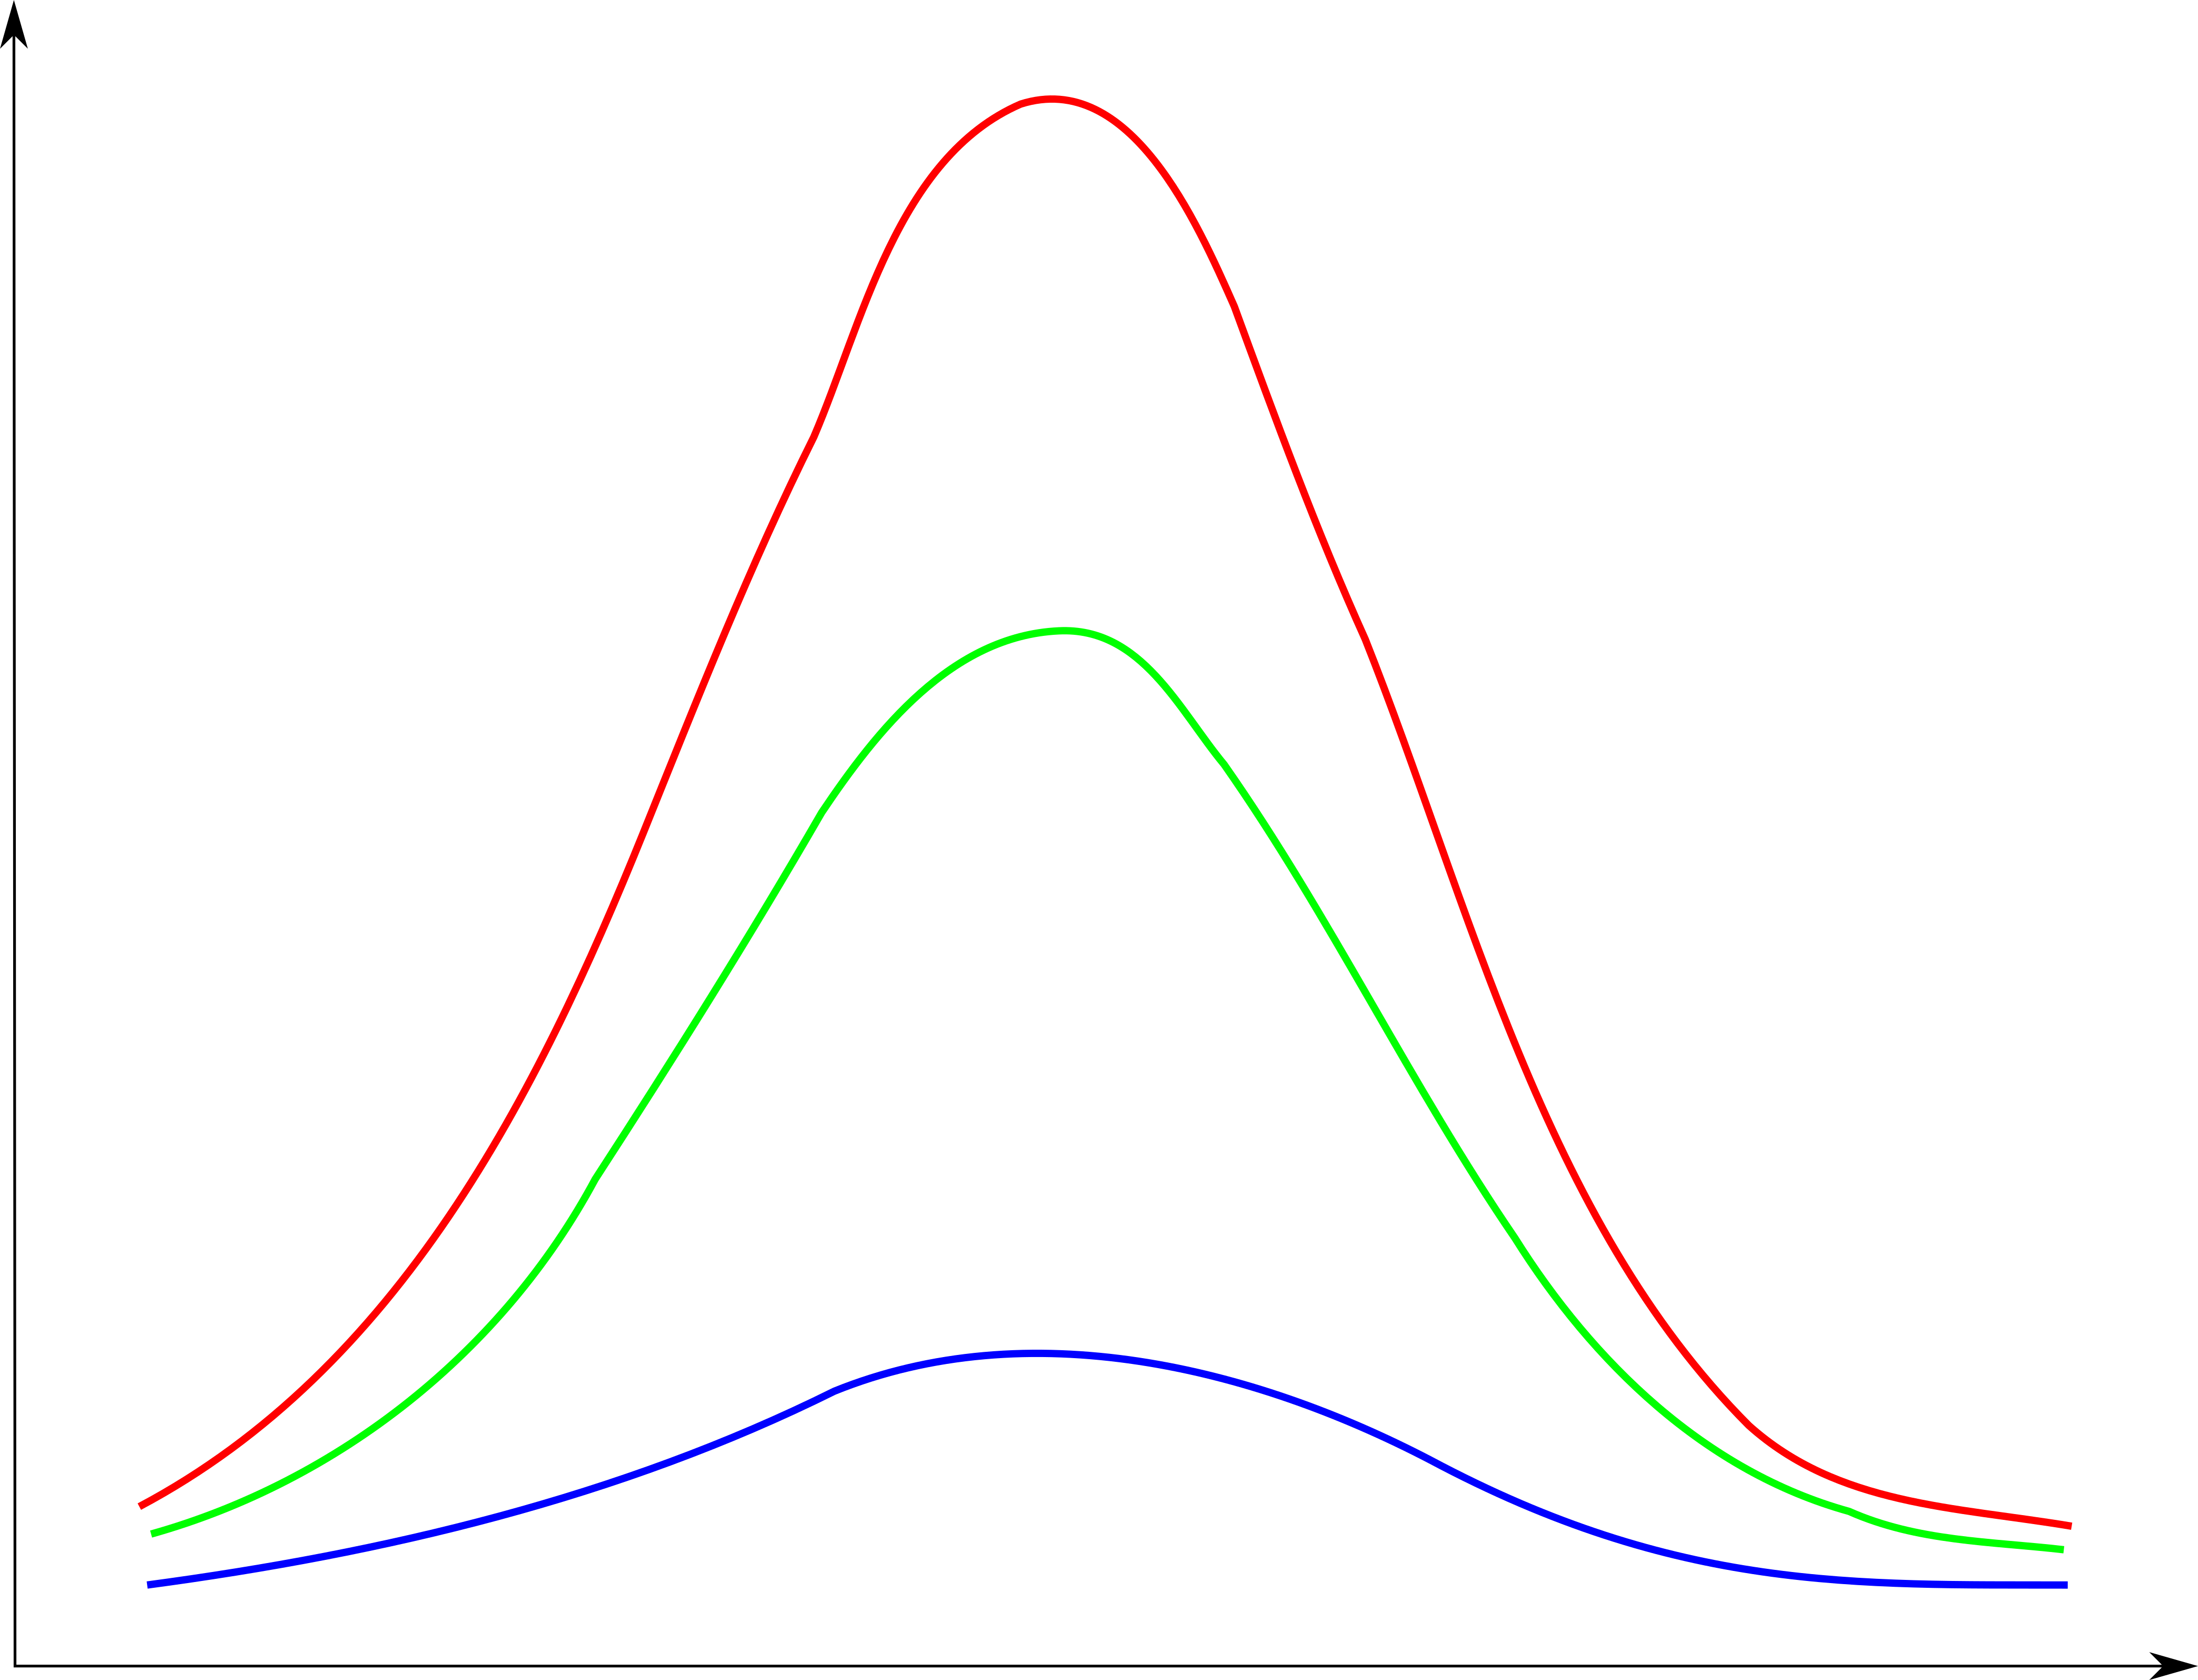
\includegraphics[width=0.5\linewidth]{./images/kurtosis.png}
	\caption{Normal Distribution with Kurtosis}
	\label{figure_kurtosis}
\end{figure}
\noindent
As can be seen in figure \ref{figure_kurtosis} the  three curves have the same spread but have different peaks. The curve with the highest peak will have the highest kurtosis. \textbf{Thus we can say that kurtosis is a measure of the peakedness of the data.}
\\
\\
At this point a further understanding of kurtosis is not required hence will proceed further without touching upon the formulae for kurtosis.

\vfill
\pagebreak

\subsection{Standard Normal Distribution}

Before the discovery of computers, a lot of calculation were done with hands, PDF for Normal Distribution were also one such calculations. However due to the complexity of the calculation, table were formed with pre-calculated values. However these tables are only valid for \textbf{standard normal distribution}.
\\
\\
\textbf{A Standard Normal Distribution is Normal Distribution with 0 as mean and standard deviation of 1}. To convert a normal distribution to standard normal distribution we need to calculate the z-score of each data point and plot the density against these z-scores instead of data points as shown in figure \ref{figure_normal_example_z}
\begin{figure}[H]
	\centering
	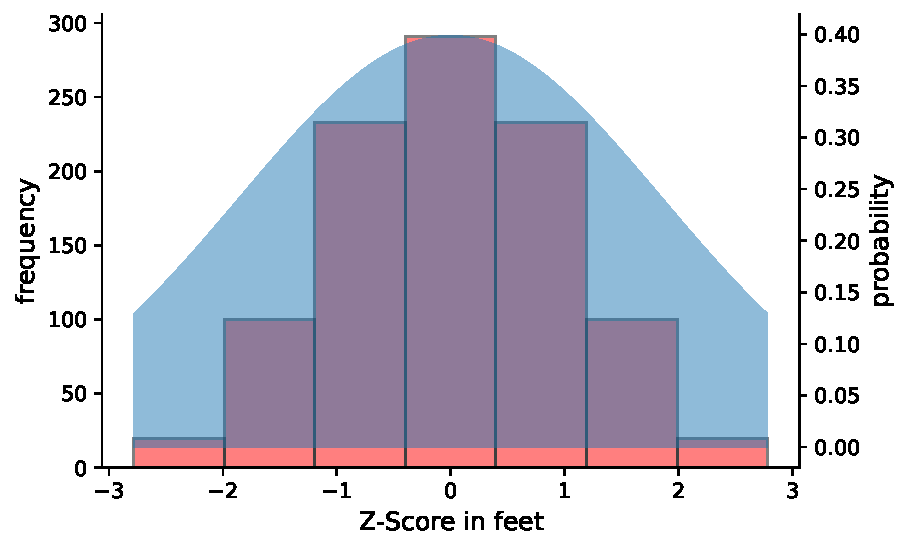
\includegraphics[width=0.5\linewidth]{./images/normal_example_z.pdf}
	\caption{Standard Normal Distribution}
	\label{figure_normal_example_z}
\end{figure}

\end{document}